
% this file is called up by thesis.tex
% content in this file will be fed into the main document

%: ----------------------- introduction file header -----------------------
\begin{savequote}[50mm]
The logic of validation allows us to move between the two limits of dogmatism and skepticism. 
\qauthor{Paul Ricoeur}
\end{savequote}


\chapter{Resultados de la investigación}
\label{cha:Validation of the methodology}

% the code below specifies where the figures are stored
\ifpdf
    \graphicspath{{5_experiments_and_results/figures/PNG/}{5_experiments_and_results/figures/PDF/}{5_experiments_and_results/figures/}}
\else
    \graphicspath{{5_experiments_and_results/figures/EPS/}{5_experiments_and_results/figures/}}
\fi


%------------------------------------------------------------------------- 

En este capítulo se evalúa si los objetivos de esta tesis se han alcanzado, es decir, la idoneidad del método propuesto para la evaluación de competencias genéricas, así como las herramientas que lo implementan.

El capítulo comienza con la descripción de las herramientas que implementan el método DBA y su ilustración con varios ejemplos. En segundo lugar, se presentan los estudios de caso en los que se ha implementado el método. En tercer lugar, se analizan los cuestionarios de evaluación y sus resultados. En cuarto lugar, se presentan las contribuciones surgidas de esta tesis doctoral. En último lugar, el capítulo termina con la discusión y las conclusiones del proceso de evaluación.

\section{Introducción}

	Para evaluar la idoneidad del método DBA se han implementado tres herramientas que se han utilizado en otros tantos entornos educativos. El trabajo comenzó en el curso 2011-12, cuando se desarrolló una herramienta web para la evaluación de competencias genéricas y específicas a partir del trabajo de los estudiantes en un wiki basado en MediaWiki. Esta aplicación se describe en los  antecedentes (sección~\ref{subcha:antecedentes}). En el siguiente curso se desarrolló una herramienta de tipo DSL para la evaluación de competencias genéricas a partir de la actividad generada por los estudiantes en el VLE (apartado~\ref{subcha:evc}). La última herramienta desarrollada también es de tipo DSL y se utilizó para la evaluación de competencias genéricas a partir de la actividad generada por los estudiantes en un mundo virtual (apartado~\ref{subcha:evs}). 

%En los antecedentes se trabaja en la extracción de indicadores sobre un wiki de MediaWiki, mientras que después se presentan dos DSLs para la extracción de indicadores. El primero de ellos a partir de los registros de un VLE (Moodle), mientras que el segundo lo hace a partir de los registros de un mundo virtual basado en OpenSim.



%	El método DBA se ha utilizado en la extracción de competencias genéricas de tres entornos educativos virtuales. Para ello se ha implementado una herramienta diferente para cada entorno. 

Las herramientas se utilizaron en varias experiencias para la evaluación de competencias genéricas en asignaturas de la Universidad de Cádiz. Estas experiencias se presentan en diferentes casos de estudio que han sido después presentados en congresos y publicados en revistas.

Por último se realizó un cuestionario para que expertos en el dominio evaluasen la idoneidad del método y la herramienta. Ambos fueron presentados a varios colectivos relacionados con la docencia y las TIC, que tras asistir a los cursos y talleres en los que se presentaron, recibieron una invitación para completar el cuestionario de evaluación.


\section{Antecedentes} \label{subcha:antecedentes}

En los antecedentes se presenta \emph{AssessMediaWiki} (AMW)\footnote{http://assessmediawiki.forja.rediris.es}, una herramienta que se desarrolló para realizar un evaluación cualitativa del trabajo de los estudiantes en el wiki y que surgió para complementar el análisis que realizaba la herramienta \emph{StatMediaWiki} (SMW)\footnote{http://statmediawiki.forja.rediris.es/}. SMW es una herramienta que realiza un análisis meramente cuantitativo de las contribuciones de los estudiantes en el wiki.
% SMW realizaba un análisis de las contribuciones de los estudiantes en el wiki meramente cuantitativo, pero que en su aplicación se topó con algunos inconvenientes que requeríanz una aproximación cualitativa.

El capítulo comienza con una introducción a la problemática surgida con los wikis, a continuación se presenta AMW y se finaliza con las conclusiones.

% SEGUIR POR AQUÍ. VER CÓMO ENCAJAR LO DE ARRIBA Y LO DE ABAJO.

\subsection{Introducción}

	El uso educacional de los wikis para las experiencias de trabajo colaborativo está en auge debido a las numerosas ventajas que aporta sobre los modelos tradicionales~\cite{elgort2008wiki}. Algunas de las ventajas sobre los medios tradicionales, ya sean en formato impreso o en documentos digitales, es que éstos no llevan un registro de ediciones, no facilitan la colaboración distribuida y asíncrona y no pueden ser monitorizados por el docente mientras los estudiantes completan el trabajo.

	Para evaluar el trabajo final de un grupo de estudiantes en una página del wiki nos bastaría con leer la última versión de dicha página, como hacíamos con los métodos tradicionales. Pero una de las características más interesantes de los wikis es que no sólo almacenan la información de la versión final de cada documento, sino que también almacenan todas las versiones intermedias creadas como resultado de las contribuciones hechas por cada usuario~\cite{trentin2009using}. Esto lo consigue manteniendo un registro con las diferencias entre las ediciones consecutivas de las páginas, registro que se podría utilizar para la obtención de indicadores de diferentes competencias~\cite{ortega2011new}. Las páginas creadas de manera colaborativa podrían ser evaluadas considerando la contribución de cada autor y las dinámicas de grupo en la creación de la página en tiempo real. Por desgracia, realizar una evaluación detallada de cada contribución realizada en el wiki es imposible de abordar cuando hay muchos usuarios y éstos participan activamente.

	En un proyecto anterior, para poder evaluar el trabajo de los estudiantes en las páginas de un wiki se desarrolló SMW, una herramienta que proporciona al docente información cuantitativa sobre la distribución del trabajo de los estudiantes en las páginas del wiki, es decir, qué parte del trabajo realizado en una página del wiki corresponde a cada estudiante~\cite{duarte2012wikis}.  A partir de esa información cuantitativa se midieron las competencias de la adaptación al cambio, el trabajo en equipo, el aprendizaje y la innovación. Sin embargo, el aspecto cualitativo quedó fuera, ya que el experimento sólo consideró el número, el momento y el tamaño de las contribuciones~\cite{palomo2014assessment}.

	Para completar el análisis cuantitativo proporcionado por SMW con un análisis cualitativo y medir el desempeño en otras competencias genéricas se desarrolla AMW. AMW es una herramienta para realizar una evaluación escalable y cualitativa del trabajo realizado en el wiki mediante procedimientos de autoevaluación, evaluación entre iguales y evaluación del docente.

		\subsection{AssessMediaWiki (AMW)}

		AMW es una aplicación web de código abierto que, al conectarse a una instalación MediaWiki, proporciona procedimientos de autoevaluación, evaluación entre iguales y evaluación del docente, a la vez que mantiene información sobre esas evaluaciones. AMW pone a disposición de los estudiantes una rúbrica previamente definida por el docente para que realicen la evaluación (figura~\ref{fig:AmwRubrica}). 

\begin{figure}
  \begin{center}
    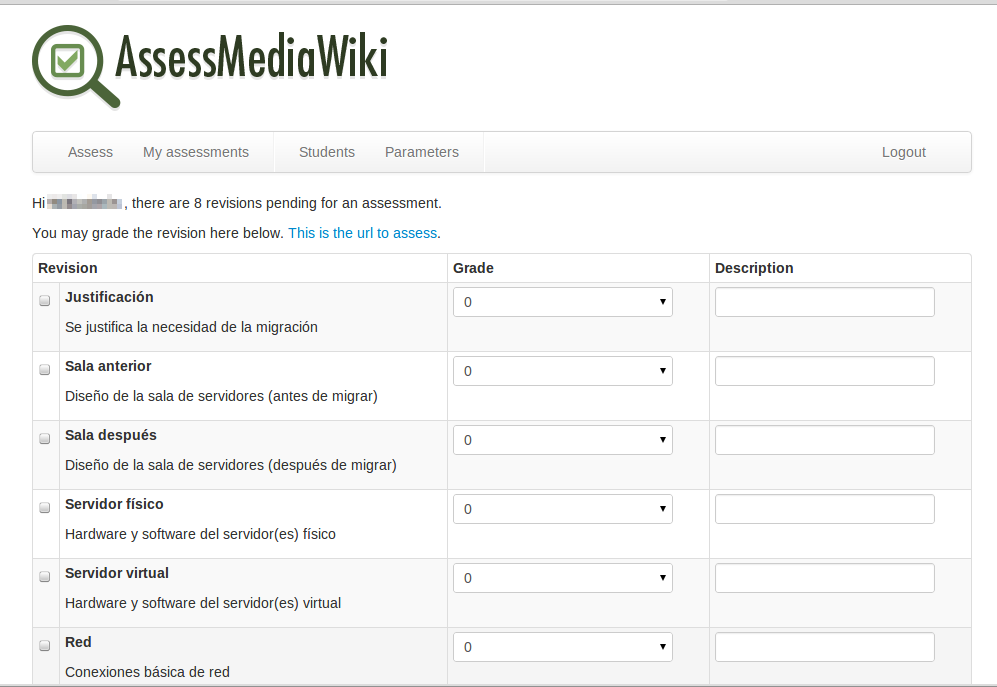
\includegraphics[scale=0.3]{AmwRubrica.png}
  \end{center}
  \caption{Rúbrica de AMW}
  \label{fig:AmwRubrica}
\end{figure}

		AMW implementa dos roles de usuario distintos: supervisores y estudiantes. Los estudiantes pueden elegir entre distintas opciones: evaluar una revisión, comprobar sus propias aportaciones evaluadas y verificar las evaluaciones ya enviadas. Por otro lado, los supervisores tienen un mayor número de opciones, como definir la rúbrica que los estudiantes deberán completar al realizar sus evaluaciones, modificar los parámetros de los programas o supervisar las evaluaciones que los estudiantes vayan haciendo. AMW implementa una función de selección parcialmente aleatoria. Cuando un estudiante va a realizar una evaluación, el sistema elige automáticamente una de entre el 30\percentage{ }de las más significativas que aún no han sido evaluadas.

		Al revisar sus evaluaciones, los estudiantes puede revisar las notas recibidas y sus justificaciones, así como ver a qué contribución en particular se refiere (figura~\ref{fig:AmwFormative}). Si el estudiante no está de acuerdo con la calificación puede replicar utilizando para ello una rúbrica similar a la que se utilizó en su evaluación, indicando las calificaciones que considera que merece y sus correspondientes justificaciones. Después el docente revisará la disputa y pondrá la nota definitiva.

\begin{figure}
  \begin{center}
    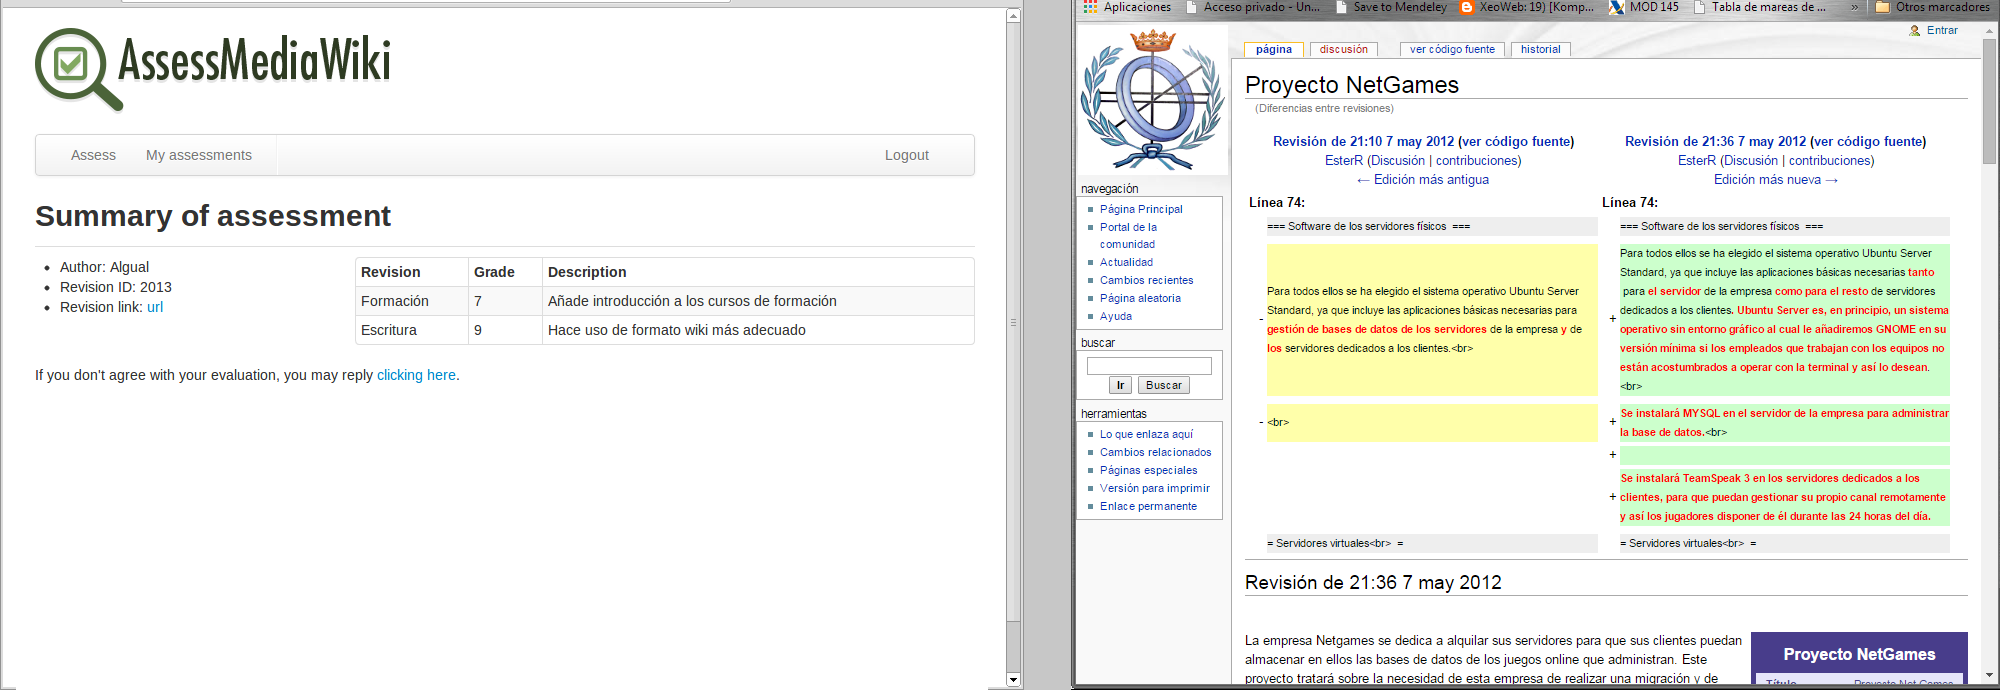
\includegraphics[scale=0.19]{AmwFormative.png}
  \end{center}
  \caption{Ejemplo de retroalimentación formativa y la contribución de wiki evaluada}
  \label{fig:AmwFormative}
\end{figure}

			\subsubsection{Ejemplo de uso}

			El método para la evaluación del trabajo y las competencias desempeñadas en el wiki consta de dos partes: una primera parte en la que lo que se evalúa es el trabajo del wiki (A), basada en procedimientos de autoevaluación, evaluación entre iguales y evaluación del docente; y una segunda parte en la que se evalúan las competencias genéricas (B) y en la que se pone en práctica el \emph{ciclo de contraste de hipótesis}.

			\paragraph*{A. Evaluación del trabajo en el wiki.}

			El método para la evaluación del trabajo en el wiki se divide también en tres fases: una primera fase en la que los estudiantes realizan sus trabajos en las páginas del wiki, una segunda fase de evaluación y una tercera fase de revisión del docente. En la figura~\ref{fig:AmwDiagram} puede verse un diagrama de flujo de trabajo que muestra cada una de las fases del método de evaluación realizado sobre una página del wiki en la que participan varios estudiantes y el docente. A continuación se describen cada una de estas fases.

\begin{figure}
  \begin{center}
    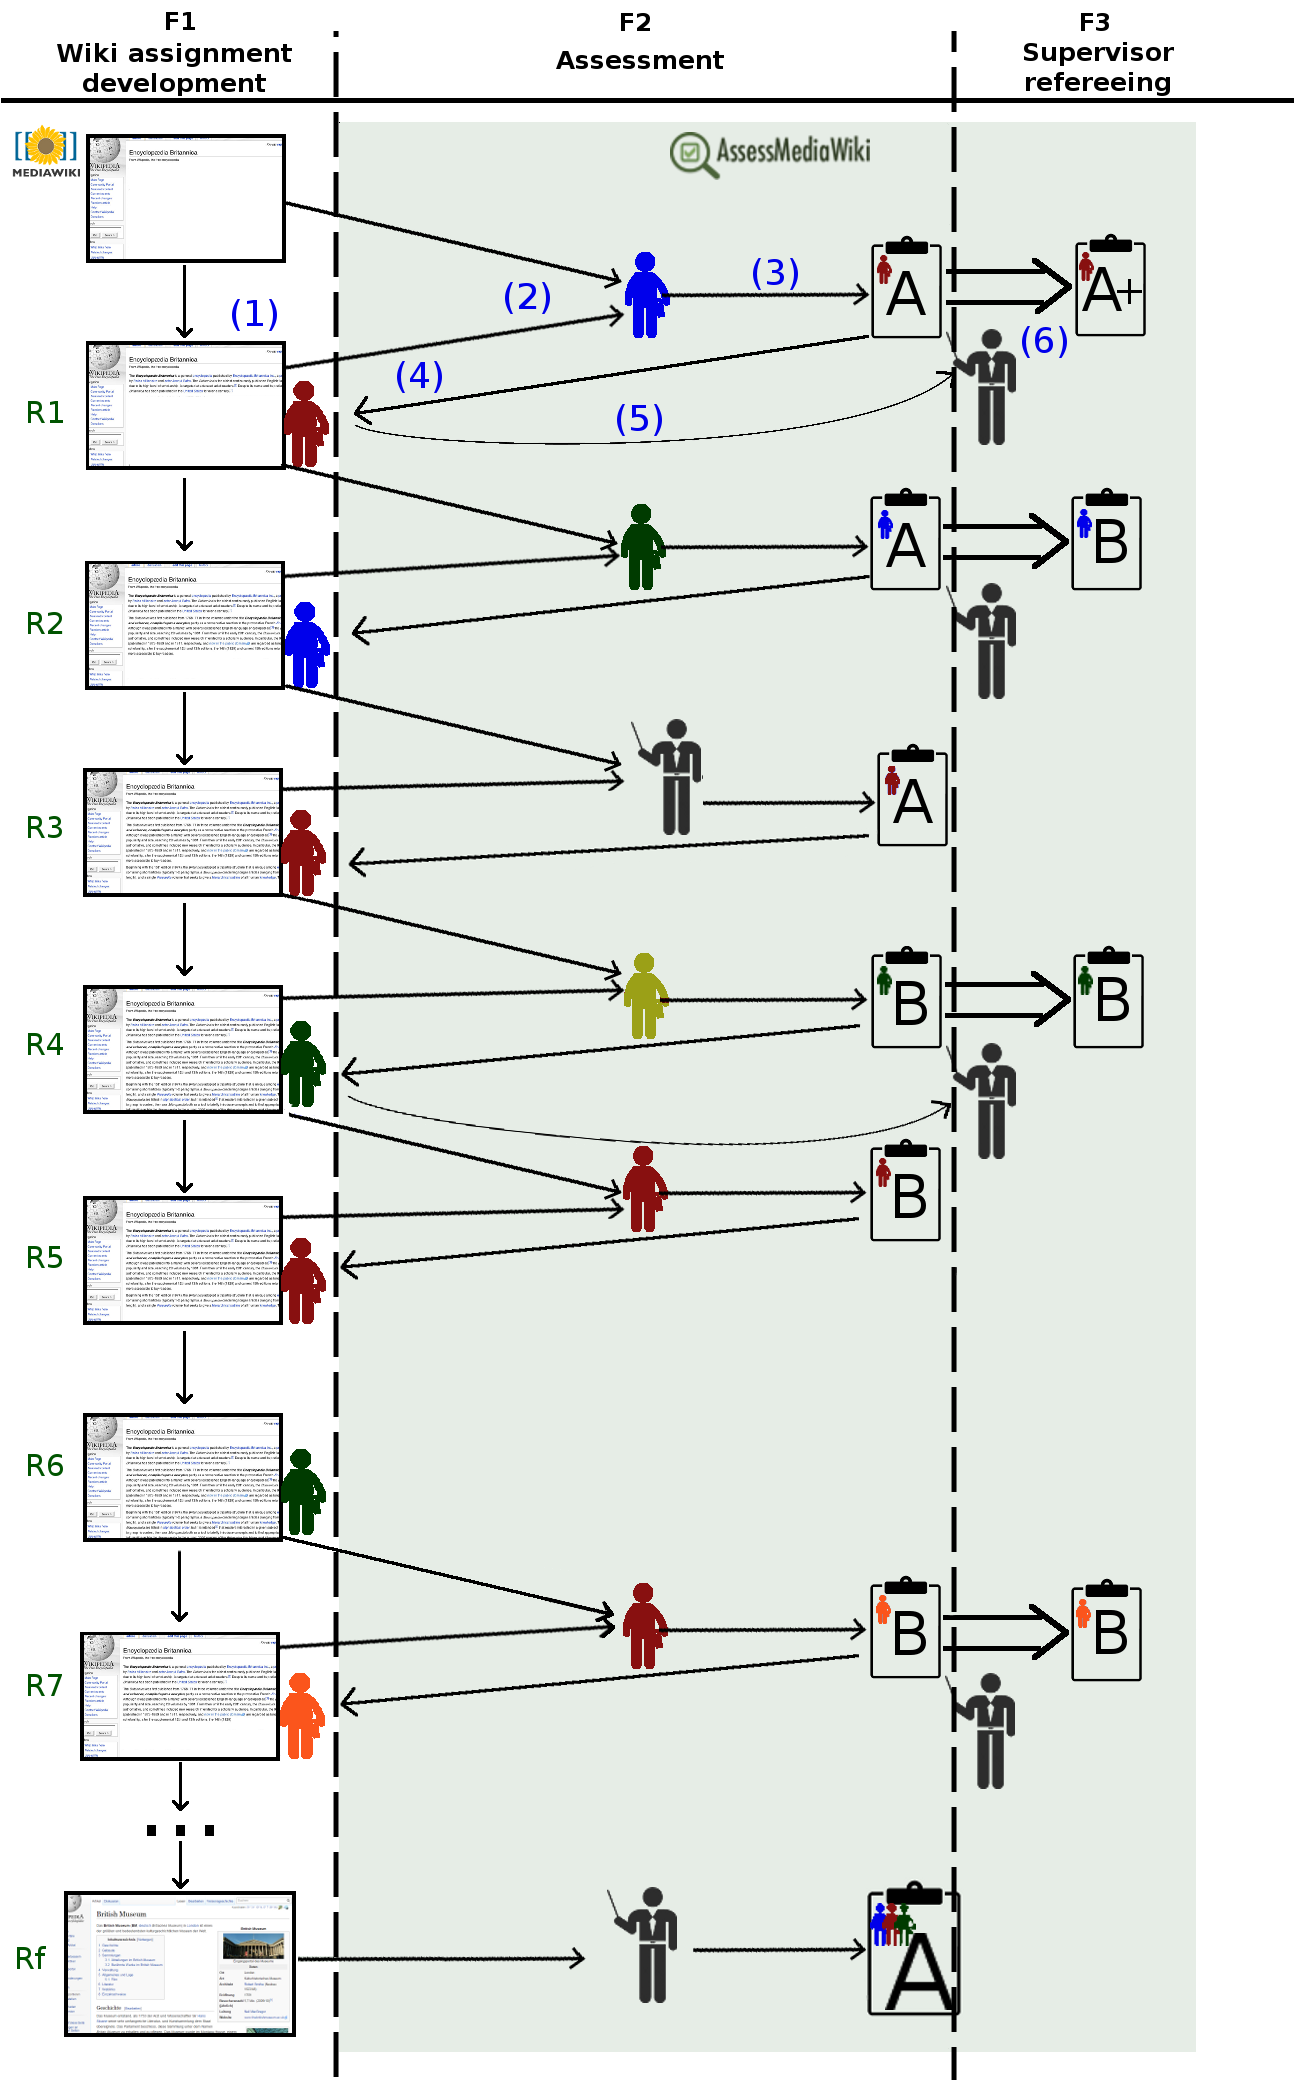
\includegraphics[scale=0.28]{AmwDiagram.png}
  \end{center}
  \caption{Ejemplo de flujo de trabajo para la evaluación cualitativa del wiki utilizando AMW}
  \label{fig:AmwDiagram}
\end{figure}

			\subparagraph*{Fase 1: Desarrollo del trabajo en el wiki.}

			Esta fase se representa en la columna de la izquierda de la figura~\ref{fig:AmwDiagram}, y es en la que los estudiantes realizan el trabajo en las páginas del wiki. Normalmente, cada grupo de estudiantes tendrá que desarrollar su trabajo en una página del wiki. En la zona más alta de la columna se representa el comienzo del trabajo con una página en blanco. El autor de cada contribución se muestra con una figura de color junto a la misma. Para comenzar, el usuario de color rojo crea una página vacía (\emph{R1}). Después, el usuario azul añade contenido a la página (\emph{R2}). En tercer lugar, el usuario rojo modifica de nuevo la página añadiendo texto a la versión dejada anteriormente por el usuario azul (\emph{R3}) y así sucesivamente. Esta fase termina cuando llega la fecha marcada por el docente para que los trabajos estén finalizados (\emph{Rf} es la versión final de la página).

			Puede verse que, aunque los estudiantes responsables de la página de ejemplo del wiki fuesen el rojo, el azul y el verde, otros estudiantes, como el naranja en la revisión séptima, podrían contribuir a la página del wiki. En ese caso, los miembros del grupo y responsables de la página deben decidir si la contribución debe conservarse o no.

			\subparagraph*{Fase 2: Evaluación.}

			Esta fase se muestra en la columna central y comprende las siguientes actividades:

			\begin{itemize}
				\item \emph{Autoevaluación, evaluación entre iguales y evaluación del docente}. Las contribuciones a ser evaluadas se asignan a los estudiantes.  Cada contribución es la diferencia entre dos revisiones consecutivas de una página del wiki. El estudiante encargado de evaluar dicha contribución se representa en el gráfico como un usuario coloreado que recibe dos flechas de las revisiones, una de la revisión anterior a la contribución y otra de la revisión que incorpora ya la contribución. Para la evaluación los estudiantes utilizan una rúbrica definida por el docente. Cada contribución sólo se refiere a una contribución atómica de las realizadas a una página del wiki por un único estudiante, por lo que dicha contribución podría ser utilizada como un indicador de la contribución al wiki de dicho estudiante. El estudiante que realizó cada contribución se representa con una figura pegada a la revisión de la página en cada momento.
Por ejemplo, en la primera evaluación, se asigna la contribución realizada a la página del wiki por el estudiante rojo (\emph{1}) al estudiante azul. El estudiante azul comprueba ambas versiones para ver las diferencias entre ambas versiones (\emph{2}) y realiza la evaluación completando la rúbrica proporcionada por el docente (\emph{3}).
Cabe destacar también otras situaciones interesantes. En la versión \emph{R5} de la página vemos como se realiza una autoevaluación, ya que el estudiante rojo, autor de la versión, es el mismo que tiene que evaluar su contribución. Vemos también que en \emph{R3} es el docente el que realiza la evaluación de la contribución del estudiante rojo. Esto puede deberse a que el estudiante manualmente detecta una contribución que considera oportuna evaluar o a que, utilizando la herramienta SMW, detecta un comportamiento extraño en el wiki y quiere contrastar la situación. 
Puede verse también que hay contribuciones que no reciben evaluación alguna, como ocurre con \emph{R6}. Está claro que sería deseable que todas las contribuciones significativas fueran evaluadas, pero no es escalable.
				\item \emph{Revisión de las evaluaciones recibidas}. Los estudiantes pueden revisar las evaluaciones recibidas. Ellos pueden no sólo ver las notas que han recibido con las justificaciones y comentarios que añadieron sus evaluadores, sino también el enlace a la contribución. De esta forma, los estudiantes evaluados reciben una retroalimentación formativa. En la primera de las evaluaciones del diagrama de ejemplo puede verse como el estudiante rojo puede ver su evaluación (\emph{4}).
				\item \emph{Réplica}. Si el estudiante evaluado no está de acuerdo con la evaluación recibida tiene la opción de replicarla justificando el motivo de dicha réplica. En el diagrama de ejemplo puede verse como el estudiante rojo considera no apropiada su evaluación y realiza una réplica (\emph{5}). El docente deberá resolver la réplica en la siguiente etapa.
				\item \emph{Evaluación final del wiki}. El docente evalúa la versión final de la página del wiki desarrollada por cada grupo de estudiantes. Esta evaluación es necesaria ya que el objetivo principal de la tarea es que los estudiantes realicen un buen trabajo en una página del wiki. Como cualquier otra tarea, deberá ser evaluada por el docente conforme al programa de estudios. Además, algunos de los criterios de evaluación sólo pueden ser evaluados en la versión final de la página, como por ejemplo, la coherencia del texto. De esta forma, aquellas contribuciones del wiki descartadas por la función de selección serán ahora implícitamente evaluadas ya que están integradas en el entregable final. Puede verse la evaluación al final del diagrama de ejemplo (\emph{Rf}), y cómo afecta al grupo de estudiantes completo.
\end{itemize}

			El diagrama no recoge algunas situaciones que también podrían darse. Por ejemplo, alguna contribución podría ser evaluada por más de un usuario, ya fuera otro estudiante o el docente. También, para simplificar, el diagrama sólo muestra una calificación para la contribución (A, A+, B, ... etc.), pero las evaluaciones son multidimensionales.

			Un componente interesante de nuestro algoritmo es qué contribución wiki podrá ser asignada a cada estudiante para su evaluación. Es lo que llamamos \emph{función de selección}, y tiene varios aspectos a tener en cuenta:

			\begin{itemize}
				\item \emph{¿Debería cierta contribución en el wiki ser evaluada por más de un estudiante?} En realidad, tener varias evaluaciones de estudiantes diferentes sobre una misma contribución podría ser interesante para perfeccionar su evaluación y podría proporcionar información al docente para evaluar no sólo al estudiante autor de la contribución, sino también a los evaluadores. De hecho, el número de contribuciones a ser evaluadas es dependiente del objetivo del experimento y su configuración. Cuánto más grande sea el experimento, más contribuciones susceptibles de ser evaluadas tendrá. Sin embargo, el número de evaluaciones que un estudiante puede realizar es limitado (para que siga siendo formativo). Por lo que cada evaluación adicional a la misma contribución provocará que otras contribuciones sean peor evaluadas o que no lo sean.
				\item \emph{¿Qué contribuciones deberían ser evaluadas?} La importancia de evaluar cada contribución puede variar. Por ejemplo, evaluar al menos una mínima cantidad de contribuciones por cada estudiante, página o categoría sería interesante. Pero algunas contribuciones que añadan ciertas características al trabajo pueden ser relevantes o informativas sobre el trabajo realizado por un estudiante. Por ejemplo, aunque las contribuciones que añadan gran cantidad de texto suelan ser más interesantes que las contribuciones pequeñas, una contribución pequeña puede ir relacionada con el cambio de sentido de alguna frase o párrafo. De cualquier forma, un estudiante puede solicitar que una contribución en particular sea evaluada, aunque ésta quede fuera de la función de selección.
				\item \emph{¿Quién evalúa cada contribución?} Depende de la importancia que se quiera dar a la autoevaluación, la evaluación del compañero y la del docente. De nuevo, se debería equilibrar el esfuerzo requerido y el detalle a exigir en las evaluaciones.
			\end{itemize}


			\subparagraph*{Fase 3: Revisión del docente.}

			En esta última columna se representan dos actividades que corresponden al docente:

			\begin{itemize}
				\item Resolución de las réplicas: el docente revisa las réplicas indicando si proceden o no. En caso de que procedan, modifica la calificación. En el diagrama se puede ver como en la primera contribución, el estudiante rojo realiza una réplica (\emph{5}) sobre la evaluación reciba por el usuario azul (\emph{3}). El docente revisa la réplica, la considera apropiada y modifica la calificación (\emph{6}). En un segundo ejemplo, en la evaluación realizada por el estudiante de color amarillo sobre la contribución realizada por el usuario de color verde puede verse como el docente no acepta la réplica realizada por este último, y mantiene la calificación otorgada inicialmente por el estudiante amarillo.
				\item Revisión de evaluaciones no replicadas: el docente puede revisar aleatoriamente otras evaluaciones realizadas por los estudiantes que no hayan sido replicadas. En el diagrama puede verse como el docente revisa las evaluaciones realizadas sobre las contribuciones representadas en \emph{R2} y en \emph{R7}, disminuyendo la calificación de la primera y manteniendo la segunda.
			\end{itemize}

			\paragraph*{B. Evaluación de competencias genéricas}

			El método para la evaluación de competencias genéricas se basa en el \emph{ciclo de contraste de hipótesis} (véase sección~\ref{cha:met-sec:dba}). En la figura~\ref{fig:AmwDiagram2} puede verse la descripción del ciclo para el caso de AMW. Esta evaluación se puede llevar a cabo durante o después de que los estudiantes hayan realizado su trabajo en el wiki y sus evaluaciones con AMW. Evidentemente, cuánto más avanzado esté el trabajo más datos habrá para analizar. 

			El ciclo comienza con el diseño de un indicador por parte del docente que podría plasmar en una hoja de cálculo a partir de los datos que recibirá de las evaluaciones (a). A continuación, el docente realiza la petición a AMW que le proporcionará los datos (b). AMW consulta y procesa los datos en las bases de datos de MediaWiki y AMW (c) y se los envía al docente (d). El docente los integra en la hoja de cálculo previamente diseñada y los analiza (e). Si son válidos para la evaluación finaliza el proceso (f). Por el contrario, si necesitan algún tipo de refinamiento el docente puede rediseñar la evaluación (g) y hacer una nueva petición.

\begin{figure}
  \begin{center}
    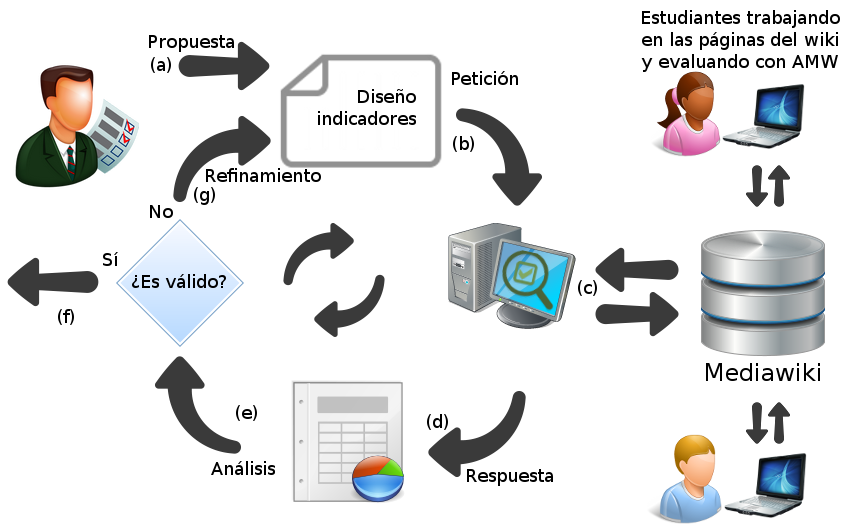
\includegraphics[scale=0.45]{AmwDiagram2.png}
  \end{center}
  \caption{Ciclo de contraste de hipótesis para la evaluación en wikis}
  \label{fig:AmwDiagram2}
\end{figure}

			\paragraph*{Indicadores de competencias genéricas}

				Los indicadores que se mencionan en este punto han sido utilizados en los estudios de caso realizados para este trabajo, pero como se ha mencionado desde un primer momento, este método proporciona indicadores y es el docente el que los utilizará para evaluar las competencias genéricas que considere oportunas.

			\subparagraph*{Trabajo en equipo.}
			El indicador considerado para el \emph{trabajo en equipo} es el \emph{ratio de miembros del equipo que trabajaron en un mismo criterio.} La rúbrica que utilizan los estudiantes para evaluar se compone de un conjunto de criterios. Cada criterio puede hacer referencia a una parte del trabajo. En todas las ediciones de un wiki no se trabajan en las mismas partes del trabajo, por lo que al ser evaluado, un estudiante puede tener nota en unos criterios y no tenerla en otros. Si más de un estudiante ha trabajado en la misma parte de una página wiki y su aportación ha sido significativa, tendrán nota en dicho criterio. Por tanto, partiendo de la cantidad de criterios que tiene un trabajo y del ratio de miembros del equipo que ha trabajado en cada criterio tendremos un indicador del \emph{trabajo en equipo}.

			\subparagraph*{Comunicación y aplicación del conocimiento.}
			El indicador considerado para la comunicación y la aplicación del conocimiento es la \emph{media de las notas recibidas por todos los miembros del grupo}. Este indicador mide la incidencia que tuvieron las contribuciones realizadas en el éxito del proyecto. Una calificación pobre en una contribución puede significar  que alguna contribución wiki obtuvo una buena nota en un cierto criterio de la rúbrica pero una mala nota en el otro (el autor de la contribución soluciona un problema y crea uno nuevo). Probablemente, esto se debió a una mala comunicación entre los miembros del equipo o poco compromiso de un determinado estudiante en el objetivo global del grupo. 

			\subparagraph*{Mantener la calidad del trabajo producido.}
			El indicador considerado para el mantenimiento de la calidad del trabajo producido es la \emph{media de las notas que cada estudiante individualmente recibió}. Unas calificaciones altas en las evaluaciones recibidas pueden significar que el trabajo que el estudiante está produciendo es de calidad. Si el estudiante produjese mucho contenido, pero este no fuese de calidad, las calificaciones no serían buenas. Es decir, sus calificaciones están teniendo en cuenta el aspecto cualitativo del trabajo y por tanto una nota alta significaría un trabajo de calidad.

			\subparagraph*{Capacidad crítica.}
			El indicador considerado para la capacidad crítica es el \emph{número de evaluaciones que el estudiante realizó con respecto al número de dichas evaluaciones cuya nota fue modificada por el docente}. Este indicador mide la competencia de un estudiante para evaluar el trabajo hecho por otros. Si recibiera un número fijado de réplicas en sus revisiones y estas fueran revisadas por el docente modificando las calificaciones, podríamos considerar que dicho estudiante no ha desempeñado bien dicha competencia.

			En la tabla~\ref{tab:ResumenIndicadoresCualiCuanti} puede verse una comparación entre los indicadores considerados a partir de la evaluación cualitativa que se realizaría con AMW y los que se obtienen a partir de la evaluación cuantitativa realizada con SMW.

\begin{table}
  \begin{center}
  \begin{tabular}{| m{3.2cm} | >{\raggedright}m{4.9cm} | m{5.1cm} |}
    \hline 
    \multirow{2}{*}{COMPETENCIAS}  & INDICADORES  & INDICADORES  \\
      &  CUALITATIVOS  &  CUANTITATIVOS \\
    \hline
    \hline
    Trabajo en equipo  & Ratio de miembros del equipo que trabajaron en un mismo criterio  & Ratio de miembros del equipo que contribuyeron a una misma página del wiki en las páginas de su proyecto \\
    \hline
    Comunicación y aplicación del conocimiento  & Media de las notas recibidas por todos los miembros del grupo  & Porcentaje de miembros del equipo que contribuyeron al menos a un 20\percentage{ }del trabajo realizado \\
    \hline
    Mantener la calidad del trabajo producido  & Media de las notas que cada estudiante individualmente recibió  & Contribución individual en bytes \\
    \hline
    Capacidad crítica  & Número de evaluaciones que el estudiante realizó con respecto al número de dichas evaluaciones cuya nota fue modificada por el docente  & No considerada \\
    \hline
  \end{tabular}
\end{center}
\caption{Resumen de las competencias evaluadas para cada tipo de indicador}
\label{tab:ResumenIndicadoresCualiCuanti}
\end{table}

			\subsubsection{Conclusiones}

			AMW es una herramienta de evaluación asistida que proporciona un análisis cualitativo interesante, pues al análisis cuantitativo proporcionado por StatMediaWiki, se podría añadir una información cualitativa que ayudase a detectar hábitos no deseados de los estudiantes. Por ejemplo, la contribución de un estudiante que copiase y pegase una gran cantidad de texto en una página del wiki sería considerada a efectos cuantitavos como una contribución de peso. Sin embargo, desde un punto de vista cualitativo, podría detectarse que la contribución había sido plagiada de internet con el fin de engañar al sistema.

			Sin embargo, en la aplicación de AMW nos encontramos con que se dan algunos de los problemas detectados en la revisión de la literatura para este tipo de herramientas de evaluación asistida. En primer lugar, delegar la evaluación en los estudiantes genera situaciones de subjetividad, pues pueden existir apartados en la rúbrica que los estudiantes interpreten o valoren de forma diferente. Y en segundo lugar, como vemos en el diagrama, el profesorado también revisa las evaluaciones de sus estudiantes, y más aún si estos replican, con lo que los problemas de escalabilidad también aparecerían.


%\section{Herramientas}
\section{Lenguajes de dominio}

		A continuación se presentan los dos DSL que se han desarrollado para la implementación del método, cada uno aplicable a un contexto diferente. En el apartado~\ref{subcha:evc} se presenta el primer DSL, orientado para obtener indicadores de los VLEs, mientras que en el apartado~\ref{subcha:evs} se presenta el segundo DSL, orientado a los mundos virtuales.

% TIC https://consultasescritura.wordpress.com/2013/03/14/tic-tics-tics-o-tic/

%	\subsection{Lenguajes de dominio}

%		Un DSL es un pequeño lenguaje de programación de gran potencia expresiva que se enfoca a un dominio particular. Los beneficios de utilizar un DSL son~\cite{vanDeursen:2000}:
%		\begin{itemize}
%			\item La solución a los problemas pueden ser expresados en un idioma y al nivel de abstracción del dominio del problema, y como consecuencia, los expertos en el dominio pueden entenderlo, validarlo, modificarlo y desarrollar sus propias soluciones.
%			\item Los programas son concisos, autodocumentados en gran medida y reutilizables para diferentes propósitos.
%			\item Mejora la productividad, la fiabilidad, la mantenibilidad y la portabilidad.
%			\item Permite la validación y optimización al nivel del dominio.
%			\item Mejora la capacidad de ser probado.
%		\end{itemize} 


		\subsection{EvalCourse (EVC) y SASQL} \label{subcha:evc}

 %, los investigadores de diferentes áreas han colaborado para extraerlos, realizar minería de datos y utilizarlos para mejorar el aprendizaje~\cite{park2015development}.

		%Además, los autores de algunos de los trabajo recopilados en el estado del arte (capítulo~\ref{cha:State of the Art}) confirman la relación entre la interacción que llevan a cabo los estudiantes en el VLE y su rendimiento en el desempeño de varias competencias genéricas~\cite{fidalgo:2015,rayon2014web}.

% ¿Quitar la cita de vanDeursen? Está antes?
	El VLE es el núcleo de los cursos virtuales, donde los estudiantes acceden para interactuar con el curso. La interacción de los estudiantes genera gran cantidad de información que queda registrada en el VLE. Esta interacción será la base para los indicadores del desempeño de competencias genéricas.

			\subsubsection{Descripción} % Análisis y diseño

			Para diseñar evaluaciones a partir de los indicadores del VLE se crea \emph{Simple Assessment Specific Query Language} (SASQL). SASQL es un lenguaje formal para la ejecución automática de consultas simples escritas utilizando un lenguaje específico de evaluación. SASQL tiene una sintaxis simple, con términos del dominio docente y orientado a la evaluación de competencias genéricas~\cite{Balderas:2013}. De esta forma, los docentes pueden fácilmente obtener indicadores almacenados de la actividad en el VLE sin requerir conocimientos técnicos en bases de datos o programación informática.

			También se implementa \emph{EvalCourse}, una herramienta informática que ejecuta instrucciones escritas en SASQL, proporcionando como resultado los indicadores solicitados. EvalCourse se comunica con el VLE para extraer la información del registro de actividad. EvalCourse\footnote{https://www.assembla.com/spaces/evalcourse} está basado en el IDE de la plataforma Eclipse, fue implementado utilizando Xtext~\cite{eysholdt2010xtext} dentro del Eclipse Modeling Framework y está disponible como software libre bajo licencia GNU GPL.

			El desarrollo de EvalCourse y SASQL se basa en los principios y técnicas de la ingeniería dirigida por modelos (MDE, del inglés Model-Driven Engineering). Este enfoque promueve la construcción de artefactos software de un modo flexible y rápido mediante el desarrollo de modelos y sus transformaciones. Nuestro DSL se define en términos de su sintaxis abstracta o metamodelo, su sintaxis concreta y un conjunto de plantillas para la transformación de modelos de consulta en código ejecutable dependiente del VLE.

\begin{figure}
  \begin{center}
    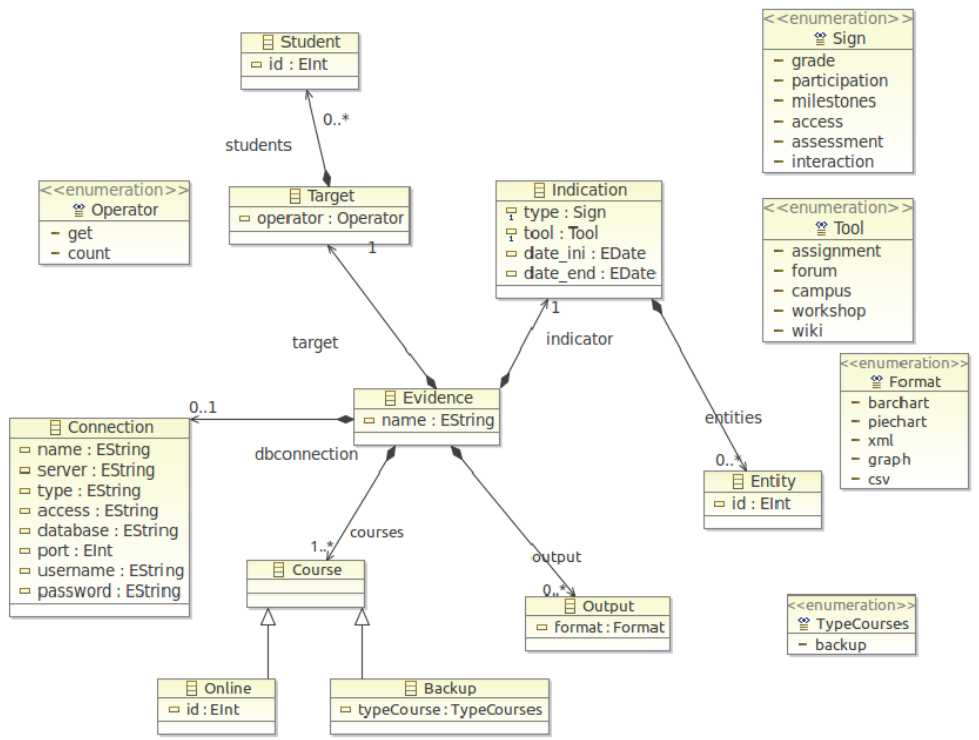
\includegraphics[scale=0.4]{EvcMetamodel.png}
  \end{center}
  \caption{Metamodelo de SASQL}
  \label{fig:EvcMetamodel}
\end{figure}

			El metamodelo de SASQL puede verse en la figura~\ref{fig:EvcMetamodel}. La entidad principal es el indicador o evidencia (\emph{evidence}). Esta evidencia se aplicará a una herramienta (\emph{tool}) que puede ser tarea (\emph{assignment}), foro (\emph{forum}), campus (\emph{campus}), taller (\emph{workshop}) o wiki (\emph{wiki}), en las que se observará un indicio (\emph{sign}), que puede ser participación (\emph{participation}), entregas (\emph{milestones}), accesos (\emph{access}), evaluaciones (\emph{assessment}), interacción (\emph{interaction}) o calificación (\emph{grade}). Además, puede actuarse sobre una actividad específica (\emph{entity}) o sobre todas las actividades de un tipo que se han dado en el VLE. La conexión a la base de datos del curso se declara en la entidad \emph{connection}. 

			En el siguiente código puede verse la sintaxis de SASQL. En la primera línea se comienza con la palabra reservada \emph{Evidence} seguida del nombre que se dará al indicador. Ese nombre será el que tengan todos los ficheros de salida. En la segunda línea se escriben los términos obligatorios \emph{get students}. En la tercera, se indica qué indicio se quiere extraer (\emph{show milestones | participation | access | interaction | assessment | grade}). En la consulta, la tercera línea se divide en dos (tercera y cuarta) para que puedan ser visualizadas todas las opciones. En la quinta, se indica sobre qué herramienta se quiere obtener el indicio (\emph{ in assignment | forum | campus | workshop | wiki [list of ids]}). También la quinta línea se divide en dos (quinta y sexta). En la séptima línea, que es opcional, se indica el rango de fechas sobre los que se extraerá la información. Y por último, en la octava se especifica si la conexión se realizará directamente a la base de datos o sobre una copia de seguridad almacenada en un fichero.

%\begin{lstlisting}[caption=Sintaxis de SASQL (las palabras reservadas se muestran resaltadas),label=code:sasqlSintax,numbers=left, captionpos=b, morekeywords={Evidence,get, students, show, milestones, participation, access, in, assignment, forum, campus, wiki, between, and, workshop, interaction, assessment, grade, from, course, backup}]


\begin{minted}[	label=Sintaxis de SASQL,
		linenos,
		frame=lines,
               	framesep=2mm]{sql}
Evidence indicator_name:
 get students 
 show milestones | participation | access 
	| interaction | assessment | grade
	| wiki [list of ids]
 between YYYY-MM-DD and YYYY-MM-DD
 from course id | backup.
\end{minted}

			El objetivo es que EvalCourse pueda ser utilizado para cualquier VLE, pero las primeras versiones han sido implementadas para funcionar en Moodle\footnote{https://moodle.org/}. Moodle es un sistema de gestión de aprendizaje de código abierto con más de 64.000 sitios registrados\footnote{https://moodle.net/stats}.


			\subsubsection{Ejemplo}

			Para evaluar las competencias genéricas el docente deberá definir los indicadores que serán extraídos de la actividad de cada estudiante en el VLE. Ilustraremos el método a partir de un ejemplo de uso de EvalCourse y su ejecución con los foros del VLE. Los foros suelen ser una de las herramientas incorporadas por los VLEs para la interacción entre los estudiantes. Es evidente que la comunicación oral es una manera muy rica de comunicarse, que proporciona múltiples signos no verbales como las expresiones faciales o el tono de voz. En contraste, las comunicaciones escritas proporcionan otras ventajas. Una de las más importantes para la educación es que el estudiante dispone de un tiempo para la reflexión. Por esta razón, podría preferirse la comunicación escrita a la oral cuando se busca un aprendizaje cognitivo~\cite{garrison1999critical}.

			La obtención de indicadores se basará en el \emph{ciclo de contraste de hipótesis} (figura~\ref{fig:EVCDiagram}). En primer lugar, es necesario que los estudiantes hayan interactuado en el VLE, de manera que su actividad haya quedado registrada. Entonces, el docente propone un diseño de evaluación mediante una consulta SASQL (a) y envía esta consulta a EvalCourse (b). EvalCourse procesa la consulta, realiza la petición a la base de datos y recoge los datos (c). Entonces EvalCourse devuelve los resultados (d). El docente analiza los resultados conforme a su propuesta de evaluación de competencias (e), terminando el proceso si éstos son válidos para él (f). Por el contrario, si los resultados no son válidos como indicadores de la competencia, entonces el docente podrá rediseñar la evaluación (g). En cualquier caso, el docente podrá reutilizar el diseño cuántas veces sea necesaria a lo largo del curso y monitorizar la evolución de los indicadores de cada estudiante.

\begin{figure}
  \begin{center}
    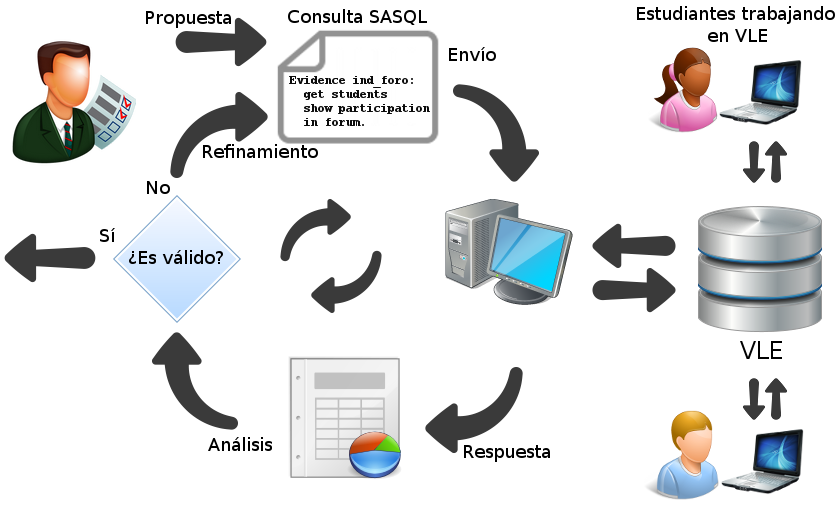
\includegraphics[scale=0.45]{EvcDiagram.png}
  \end{center}
  \caption{Ciclo de contraste de hipótesis utilizando EvalCourse}
  \label{fig:EVCDiagram}
\end{figure}

			En este ejemplo, el docente pretende obtener indicadores del uso del foro para evaluar la competencia genérica de las habilidades interpersonales. Durante el curso, los estudiantes interactuarán en el foro conforme a las instrucciones proporcionadas por el docente. Cuando lo desee, el docente podrá utilizar EvalCourse para obtener los indicadores.

% Estos indicadores deben ser publicados para que los estudiantes sepan cómo serán evaluados % FRASE ELIMINADA DEL MEDIO DEL PÁRRAFO ANTERIOR

			El docente considera que podría diseñar un indicador válido a partir del número de mensajes que ha escrito cada estudiante en un periodo de tiempo particular y plantea la siguiente hipótesis: \emph{se considerará que un estudiante ha desempeñado satisfactoriamente la competencia genérica de las habilidades interpersonales si ha escrito al menos dos mensajes en el foro}. Para ello se diseña la consulta que se muestra a continuación (consulta SASQL participaciones foro). EvalCourse procesa la consulta y devuelve los resultados que se pueden ver en la tabla~\ref{tab:EvalCourseEj1}.



%\begin{lstlisting}[caption=Consulta para obtener la participación en el foro en un periodo concreto de tiempo ,label=code:sasqlejemplo1,numbers=left, captionpos=b, morekeywords={Evidence,get, students, show, milestones, participation, access, in, assignment, forum, campus, workshop, interaction, between, and}]



\begin{minted}[	label=Consulta SASQL participaciones foro,
		linenos,
		frame=lines,
	        framesep=2mm]{pascal}
Evidence participacion_foro: 
	get students
	show participation
	in forum between 2015-10-21 and 2015-10-27.
\end{minted}


\begin{table}
	\centering
	\caption{Información sobre la participación en el foro de los estudiantes en un periodo concreto de tiempo}
	\label{tab:EvalCourseEj1}
	\begin{tabular}{|l|l|c|c|c|c|c|}
		\hline
		id & username & Debate-starter & Debate-participation & Total \\
		\hline
		\hline
		1 & student1 & 1 & 2 & 3  \\
		\hline
		2 & student2 & 0 & 4 & 4  \\
		\hline
		3 & student3 & 0 & 1 & 1  \\
		\hline
		4 & student4 & 1 & 2 & 3  \\
		\hline
		5 & student5 & 0 & 2 & 2  \\
		\hline
	\end{tabular}
\end{table}

			A la vista de los resultados, y en base a la hipótesis inicial, se podría decir que todos los estudiantes menos el 3 (\emph{student3}) habrían desempeñado correctamente la competencia. Sin embargo, el docente considera que esta primera aproximación es un poco pobre y decide completar su hipótesis de la siguiente manera: \emph{se considerará que un estudiante ha desempeñado satisfactoriamente la competencia genérica de las habilidades interpersonales si ha escrito al menos dos mensajes en el foro y ha interactuado con más de un compañero}. Para ello escribe la consulta SASQL interacciones foro.

%\begin{lstlisting}[caption=Consulta para obtener la interacción en el foro en un periodo de tiempo determinado, label=code:sasqlejemplo2,numbers=left, captionpos=b, morekeywords={Evidence,get, students, show, milestones, participation, access, in, assignment, forum, campus, workshop, interaction, between, and}]

\begin{minted}[	label=Consulta SASQL interacciones foro,
		linenos,
		frame=lines,
               	framesep=2mm]{pascal}
Evidence interacciones_foro: 
	get students
	show interaction
	in forum between 2013-10-21 and 2013-10-27.
\end{minted}


			Además del listado con las interacciones, EvalCourse proporciona varias figuras con la representación de la información. Para esta última consulta se devuelve un grafo para una mejor visualización de las interacciones (figura~\ref{fig:EvalCourseInteraccionForo}). A tenor de los resultados vemos que sólo dos de los estudiantes cumplen la segunda hipótesis (\emph{student2} y \emph{student4}). 

\begin{figure}
	\centering
	\includegraphics[width=6cm]{{EvalCourseInteraccionForo.png}}
	\caption{Interacción en el foro en un periodo de tiempo.}
	\label{fig:EvalCourseInteraccionForo}
\end{figure}

			De esta manera, el docente irá redefiniendo sus hipótesis hasta dar con los indicadores que a su juicio satisfagan la evaluación de la competencia genérica.

			\paragraph*{Propuesta de indicadores para el ejemplo}

			En este apartado se muestra una propuesta de uso de indicadores obtenidos mediante EvalCourse para la evaluación de competencias genéricas~\cite{Balderas:2015}. Pero al igual que ocurre con el resto de herramientas, estos indicadores podrían ser válidos para unos docentes y no serlos para otros, así como que habrá otras muchas formas de combinar la información del registro para obtener indicadores válidos para otras competencias genéricas.

				\paragraph*{Habilidades interpersonales}
				Para la evaluación de esta competencia genérica se propone utilizar la participación en el foro. Al crear grupos de trabajo en el VLE se puede crear un foro para cada grupo. Durante el curso se fomenta que los estudiantes intervengan en dichos foros para comunicarse entre los miembros del equipo y dejar constancia de los mensajes de cara al docente. Por tanto, si no utilizan el foro, los estudiantes no tienen calificación en esta competencia. Por ejemplo, podría fijarse que un estudiante con tres o más intervenciones en el foro tuviera una evaluación positiva en la competencia. Para obtener la información que nos permita utilizar este indicador utilizaríamos la consulta mostrada a continuación, que devolvería como resultado el listado con los mensajes iniciados, las respuestas dadas y el total de mensajes de cada estudiante en el foro, siendo este último valor el que utilizaríamos como indicador positivo para quellos estudiantes que tengan tres o más participaciones.

% label=Habilidades interpersonales en SASQL,
\begin{minted}[linenos,frame=lines,
               framesep=2mm]{pascal}
Evidence habilidades_interpersonales: 
	get students
	show participation
	in forum.
\end{minted}

				\paragraph*{Liderazgo}
				Para evaluar el liderazgo de los estudiantes se proponen también los foros creados para la comunicación de los equipos de trabajo. Para ello se podría considerar la cantidad de debates que cada estudiante ha iniciado. Por ejemplo, un estudiante que iniciara dos o más debates tendría una evaluación positiva en la competencia de liderazgo. Para obtener la información que nos permita utilizar este indicador utilizaríamos la consulta mostrada a continuación, que devolvería como resultado el listado con los mensajes iniciados, las respuestas dadas y el total de mensajes de cada estudiante en el foro, siendo el primer valor el que utilizaríamos como indicador positivo para quellos estudiantes que tengan dos o más participaciones.

% label=Liderazgo en foro con SASQL,
\begin{minted}[linenos,frame=lines,
               framesep=2mm]{pascal}
Evidence liderazgo_foro: 
	get students
	show participation
	in forum.
\end{minted}

				El wiki de Moodle también se podría prestar a la evaluación de esta competencia genérica. Si tenemos registros de un usuario que se encarga de las primeras ediciones de una página del wiki (organizando el trabajo del equipo) y registros de actividad de ese usuario tras los registros de actividad de sus compañeros (revisando el trabajo de estos), podría considerarse que ese usuario está ejerciendo una labor de líder en el equipo. Para obtener la información que nos permita utilizar este indicador utilizaríamos la consulta mostrada a continuación, que devolvería como resultado el listado con el momento y el peso de las contribuciones de cada estudiante. El docente utilizaría estos valores contrastaría los valores de los otros estudiantes para valorar si ha ejercido o no de líder.

% label=Liderazgo en wiki con SASQL,
\begin{minted}[linenos,frame=lines,
               framesep=2mm]{pascal}
Evidence liderazgo_wiki: 
	get students 
	show interaction 
	in wiki.
\end{minted}

				\paragraph*{Pensamiento crítico}
				En Moodle hay una actividad que son los talleres (\emph{workshops}). En esta actividad, los estudiantes tienen que entregar un ejercicio conforme a las instrucciones del docente que podrá ser autoevaluada o evaluada por uno o varios compañeros. Por ejemplo, podría plantearse que cada estudiante tuviera que hacer varias tareas. Una vez entregada cada tarea, el docente pondría la solución del ejercicio a disposición de los estudiantes, y cada tarea sería evaluada por dos compañeros y por el propio estudiante. Para evaluar la competencia del pensamiento crítico, el docente utilizaría para cada tarea la diferencia entre la media de las notas dadas por sus compañeros y la que se asignó el propio estudiante. Para obtener la información que nos permita utilizar este indicador utilizaríamos la consulta mostrada a continuación, que devolvería como resultado el listado de estudiantes con tres columnas adicionales, la primera con la calificación fruto de la autoevaluación y las dos siguiente de la evaluación realizada por los otros estudiantes. El docente utilizaría la diferencia entre estos valores para valorar la competencia genérica.

% label=Liderazgo en wiki con SASQL,
\begin{minted}[linenos,frame=lines,
               framesep=2mm]{pascal}
Evidence pensamiento_critico:  
	get students 
	show assessment 
	in workshop.
\end{minted}

				\paragraph*{Planificación y gestión del tiempo}
				Las tareas programadas en el VLE tienen una fecha límite de entrega. Sin embargo, el docente puede configurar la actividad para que permita envíos retrasados. El docente podría establecer un número mínimo de trabajos entregados antes de la fecha límite para considerar que esta se ha entregado a tiempo. De esta manera, un docente podría considerar que si las tareas se han entregado tarde, pero son correctas, tengan una buena calificación en lo que a las habilidades y conocimientos específicos que requería la tarea se refiere. Pero con respecto a la planificación y gestión del tiempo de ese estudiante la calificación sería negativa, dado que ha incumplido la planificación y los plazos que se acordaron a comienzos del curso. Para obtener la información que nos permita utilizar este indicador utilizaríamos la consulta mostrada a continuación, que devolvería como resultado el listado de estudiantes indicándose para cada uno la cantidad de tareas entregadas, las que ha entregado a tiempo de estas y las que han quedado pendientes. A partir de esta información el docente podrá evaluar la planificación y gestión del tiempo de sus estudiantes.

% label=Liderazgo en wiki con SASQL,
\begin{minted}[linenos,frame=lines,
               framesep=2mm]{pascal}
Evidence planificacion:  
	get students 
	show milestones 
	in assignment.
\end{minted}

		\subsection{EvalSim (EVS) y VWQL} \label{subcha:evs}

		La segunda propuesta de DSL se aplica a los mundos virtuales. Aunque muchos investigadores han reconocido la potencia educativa y motivacional de los videojuegos, hay pocos estudios empíricos que hayan investigado recientemente su impacto en el aprendizaje de los estudiantes~\cite{berns2013game}. Lo mismo se puede decir de los entornos de aprendizaje como los mundos virtuales (Second Life, OpenCobalt, etc.)~\cite{hew2010use}. Esto se debe a que normalmente no se distribuyen bajo licencia libre y, por consiguiente, los docentes no pueden analizar las interacciones de los estudiantes o analizar su impacto en el aprendizaje y en los resultados de aprendizaje~\cite{cruz2015discovering,moreno2014serious}. 

		Ante esta situación, en un trabajo previo desarrollamos nuestro propio mundo virtual, basado en OpenSim (software de código abierto)~\cite{berns2013using}. De esta forma se podría evaluar la competencia de la comunicación en una segunda lengua a partir de las interacciones llevadas a cabo por los estudiantes en el mundo virtual.

		A continuación se explicará cómo a partir de la actividad generada por los estudiantes se obtendrán indicadores para el diseño de evaluaciones de competencias genéricas.

			\subsubsection{Descripción}

			Para este trabajo se creó VWQL (\emph{Virtual Worl Query language}). VWQL es un DSL creado para obtener indicadores objetivos de OpenSim. EvalSim es el sistema que procesa las consultas de VWQL. Ha sido desarrollado bajo un enfoque MDE para modelar procesos para la obtención de los indicadores que se requieran. Fue también implementado utilizando Xtext~\cite{eysholdt2010xtext} dentro del Eclipse Modeling Framework.

			La sintaxis del lenguaje (versión beta 0.1) puede verse en el cuadro de sintaxis VWQL. La primera línea especifica el nombre del indicador (\emph{name\_of\_the\_indicator}) y se utiliza para diferenciar los diferentes archivos producidos por EvalSim. La segunda línea comienza obligatoriamente con \emph{get students} y a continuación se ha de especificar si se quiere obtener la información para todos los estudiantes que participaron en la experiencia o sólo para algunos de los que participaron (indicando sus identificadores numéricos de usuario). La última línea indica el tipo de información a extraer tras el término obligatorio \emph{show}, y esta información puede ser de alguno de los siguientes tipos:

\begin{itemize}
\item \emph{words}: número de palabras escritas en el chat de texto. Por defecto cuenta todas las palabras, a no ser que se indique un idioma, en cuyo caso únicamente muestra, de las palabras introducidas en el chat de texto, las palabras en dicho idioma.
\item \emph{sentences}: número de frases escritas en el chat de texto.
\item \emph{single}: número de frases compuestas por una sola palabra escritas en el chat de texto.
\item \emph{turns}: número de turnos empleados en chat de texto. Un turno es un conjunto de frases consecutivas escritas por el mismo usuario.
\item \emph{time}: número de minutos jugados en el mundo virtual.
\item \emph{points}: número de puntos obtenidos en el mundo virtual. La manera en que los puntos se obtengan dependerá específicamente del mundo virtual jugado.
\end{itemize}

%\begin{lstlisting}[caption=Palabras reservadas y formato de VWQL (version 0.1), label=code:reserved,numbers=left, captionpos=b, morekeywords={Evidence,get, students, show, words, sentences, turns, time, points}]
\begin{minted}[	label=Sintaxis VWQL,
		linenos,
		frame=lines,
               	framesep=2mm]{sql}
Evidence name_of_the_evidence:
    get students [id_of_the_student]
    show ( words [dict] | sentences | turns | single |
         | time | points )+
\end{minted}

			\subsubsection{Ejemplo}

			En el juego los estudiantes interactúan entre ellos por medio de un chat. Las conversaciones quedan almacenadas en la base de datos de EvalSim. Utilizando el \emph{ciclo de contraste de hipótesis} los docentes obtendrán indicadores del trabajo de sus estudiantes (figura~\ref{fig:EvsDiagram}).

\begin{figure}
  \begin{center}
    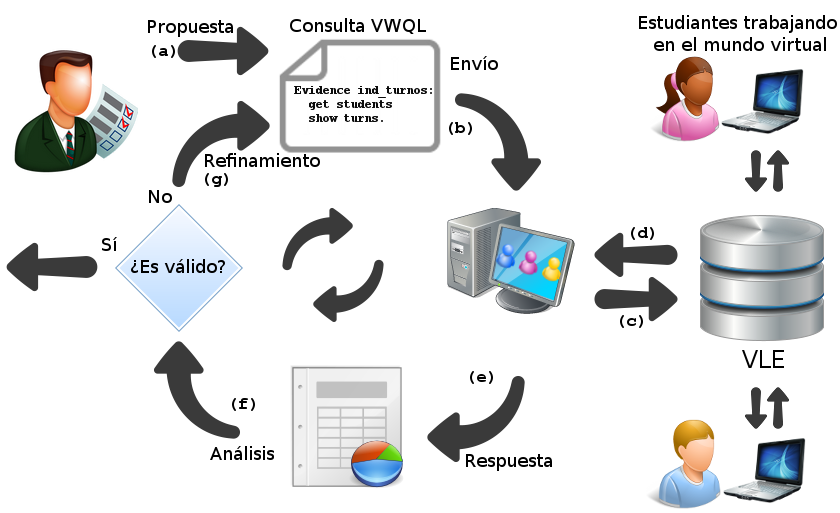
\includegraphics[scale=0.4]{EvsDiagram.png}
  \end{center}
  \caption{Ciclo de contraste de hipótesis con EvalSim}
  \label{fig:EvsDiagram}
\end{figure}

			El docente propone una evaluación (\emph{a}) que bajo su criterio le vaya a proporcionar indicadores válidos para evaluar alguna competencia genérica y la envía a EvalSim (\emph{b}). EvalSim procesa la petición y realiza la solicitud a la base de datos del mundo virtual (\emph{c}) . Una vez que recibe los datos (\emph{d}), los transforma y devuelve los resultados debidamente formateados al docente (\emph{e}). El docente los analiza, y si considera que son indicadores válidos para evaluar la competencia (\emph{f}) termina el ciclo. Sin embargo, si entiende que no les sirven o considera que debería refinarlo podría volver a diseñar una nueva evaluación (\emph{g}), reiniciándose de nuevo el ciclo.


			%\paragraph{Ejemplo de uso}

			En este ejemplo se parte de que el mundo virtual se está utilizando en una asignatura de idiomas. En un ejercicio práctico confeccionado por el docente, los estudiantes han de participar en un juego de roles (\emph{role-play}) y son advertidos de que deben explayarse en sus respuestas a fin de utilizar los recursos lingüísticos aprendidos en clase.

			Una vez que todos los estudiantes han participado el juego, el docente decide utilizar como indicador el número de frases de una sola palabra utilizada por los estudiantes. De esta manera, todos aquellos estudiantes que hayan utilizado una sola palabra para responder a alguna pregunta tendrán una evaluación negativa en el desempeño de la competencia. Puede verse el código empleado en la consulta VWQL 1.

%\begin{lstlisting}[caption=Consulta para obtener la cantidad de respuestas de una sola palabra de cada estudiante, label=code:vqwlej1,numbers=left, captionpos=b, morekeywords={Evidence,get, students, single, show, words, sentences, turns, time, points}]
\begin{minted}[label=Consulta VWQL 1,
		linenos,
		frame=lines,
               	framesep=2mm]{pascal}
Evidence respuestas_cortas:
    get students
    show single.
\end{minted}

			Como resultado a la consulta, el sistema devuelve el listado que puede verse en la tabla~\ref{tab:EvsListEj1}. A la vista de los mismos, el docente considera que hay situaciones en las que una respuesta corta podría admitirse como válida, por lo que decide admitir como mucho dos respuestas cortas en la participación de cada estudiante. Ante este enfoque, el docente considera que los estudiantes 3, 6 y 7 (\emph{student3, student6 y student7}) tuvieron un desempeño bajo en la competencia al haber empleado cuatro, cuatro y tres respuestas cortas respectivamente.

\begin{table}
	\centering
	\caption{Información sobre las respuestas de una sola palabra dadas por los estudiantes en el role-play}
	\label{tab:EvsListEj1}
	\begin{tabular}{|l|l|c|}
		\hline
		id & username & singles \\
		\hline
		\hline
		1 & student1 & 0  \\
		\hline
		2 & student2 & 1  \\
		\hline
		3 & student3 & 4  \\
		\hline
		4 & student4 & 0  \\
		\hline
		5 & student5 & 2  \\
		\hline
		6 & student6 & 4  \\
		\hline
		7 & student7 & 3  \\
		\hline
		8 & student8 & 1  \\
		\hline
	\end{tabular}
\end{table}

			Para enriquecer este indicador, el docente decide diseñar un nuevo indicador. En este caso, calculando el número de palabras por turno que escriben los estudiantes. Para ello utiliza la consulta VWQL 2. Los resultados en este caso puede verse en la tabla~\ref{tab:EvsListEj2}.

%\begin{lstlisting}[caption=Consulta para obtener las palabras por turno de cada estudiante, label=code:vqwlej2,numbers=left, captionpos=b, morekeywords={Evidence,get, students, single, show, words, sentences, turns, time, points}]
\begin{minted}[	label=Consulta VWQL 2,
		linenos,
		frame=lines,
               	framesep=2mm]{pascal}
Evidence palabras_turno:
    get students
    show words, turns.
\end{minted}

\begin{table}
	\centering
	\caption{Información sobre las palabras por turnos utilizadas por los estudiantes en el role-play}
	\label{tab:EvsListEj2}
	\begin{tabular}{|l|l|c|c|c|}
		\hline
		id & username & words & turns & words per turn \\
		\hline
		\hline
		1 & student1 & 117 & 9 & 13 \\
		\hline
		2 & student2 & 132 & 11 & 12  \\
		\hline
		3 & student3 & 63 & 9 & 7  \\
		\hline
		4 & student4 & 140 & 10 & 14  \\
		\hline
		5 & student5 & 99  & 11 & 9 \\
		\hline
		6 & student6 & 80 & 10 & 8  \\
		\hline
		7 & student7 & 72 & 9 & 8  \\
		\hline
		8 & student8 & 108 & 9 & 12   \\
		\hline
	\end{tabular}
\end{table}

			A la vista de los resultados, el docente confirma que los estudiantes 3, 6 y 7 (\emph{student3, student6 y student7}) son los que utilizan menos palabras por turno. Son estos tres estudiantes, junto con el estudiante número 5 (\emph{student5}), los únicos que bajan de 10 palabras por turno. Lo que podría ser una justificación para el docente a la hora de evaluar de manera negativa a este estudiante, ya que no sólo no llega a 10 mensajes sino que también es el único que en la consulta anterior está en el límite fijado de dos respuestas cortas.

			Como en los casos anteriores, será decisión del docente el uso que se dé a los indicadores.

			\paragraph*{Propuesta de indicadores para el ejemplo}

			El mundo virtual se ha desarrollado para asignaturas de idiomas, por lo que la competencia genérica para la que más se han utilizado los indicadores obtenidos ha sido para la \emph{habilidad para comunicarse en un segundo idioma}. No obstante, los indicadores podrían ser utilizados en la evaluación de otras competencias genéricas bajo el criterio del docente que diseña la evaluación.

% Hipótesis: un estudiante tiene dificultades para hacerse entender si necesita dos o más frases por turno para comunicarse con su compañero.

			\subparagraph*{Segundo idioma}
\begin{itemize}
\item \emph{Ritmo}: número de frases escritas por minuto. Según la experiencia desarrollada podría ser un indicador positivo o negativo del desempeño de la competencia. Si el estudiante tiene que contar una historia o expresarse sin restricción, el hecho de que escriba muchas frases por minuto es un indicador positivo de su dominio del idioma. Sin embargo, si el estudiante tiene que enviar a su compañero un mensaje concreto y tiene dificultades  para hacerse entender, puede necesitar más de una frase por minuto para hacerse entender, siendo entonces un indicador negativo.
\item \emph{Frases por turno}: número de frases escritas por turno. Igual que en el caso anterior, puede tomarse como un indicador positivo o negativo dependiendo del caso. Si el estudiante tiene un buen dominio del idioma y no hay restricción impuesta, puede ser un indicador positivo que escriba muchas frases por turno. Mientras que si necesita muchas frases para transmitir un mensaje concreto, que tenga que escribir muchas frases por turno puede ser un indicador negativo del desempeño de la competencia.
\item \emph{Palabras solas}: número de frases de una sola palabra escritas por el estudiante. Un abuso del uso de frases de una sola palabra puede ser utilizado como un indicador del bajo nivel de conocimiento del segundo idioma.
\end{itemize}

			\subparagraph*{Capacidad de aprender y mantenerse al día con el aprendizaje}
			Si un estudiante tiene dificultades para desenvolverse en el idioma, el hecho de que dedicase muchos minutos a jugar en el mundo virtual podría ser un indicador de que dicho estudiante está comprometido con su aprendizaje, y quiere mejorar. Sin embargo, si un estudiante tiene malos resultados, y además pasa pocos minutos practicando, sería un indicador negativo de esta competencia.

\section{Estudios de caso}

	Entre los cursos 2010-11 y 2014-15 se han realizado diversas experiencias para la evaluación de competencias genéricas utilizando el método DBA y las herramientas que lo implementan. A continuación se describen brevemente dichas experiencias, mientras que las publicaciones en las que se han presentado se resumen en la tabla~\ref{tab:ResumenCS} y se describen en el apartado~\ref{eva:contribuciones}.


\begin{table}
	\centering
	\caption{Resumen de publicaciones de los estudios de caso}
	\label{tab:ResumenCS}
	\begin{tabular}{|c|l|l|}
		\hline
		Estudio de caso & Congreso & Revista \\
		\hline
		\hline
		CS01 & SPDECE 2012 (\cite{Balderas:2012}) & CHB 2014 (\cite{palomo2014scalability})  \\
		\hline
		CS02 & TEEM 2013 (\cite{balderas2013generative}) & IJEE 2015 (\cite{Balderas:2015})  \\
		\hline
		CS03 & SIIE 2014 (\cite{balderas2014domain})  & IJEE 2015 (\cite{Balderas:2015}) \\
		\hline
		CS04 & TEEM 2013 (\cite{balderas2013generative})   & IJEE 2015 (\cite{Balderas:2015})  \\
		\hline
		CS05 & SIIE 2014 (\cite{balderas2014domain}) &  IJEE 2015 (\cite{Balderas:2015}) \\
		\hline
		CS06 & TEEM 2015 (\cite{balderas2015domain}) & JITR 2016 (In process) \\
		\hline
	\end{tabular}
\end{table}

	\subsection{Estudio de caso CS01}

		Este estudio se llevó a cabo en la asignatura de \emph{Administración de Sistemas Operativos} durante los cursos 2010-11 y 2011-12, con 38 y 40 estudiantes respectivamente. Esta asignatura tenía lugar en el segundo semestre del tercer (y último) curso de la titulación de Ingeniería Técnica en Informática de Sistemas. Los estudiantes tuvieron que desarrollar varias tareas durante el curso, dos de ellas en un wiki público\footnote{http://wikis.uca.es/wikiASO}. La primera consistió en un proyecto de migración de la infraestructura de red de una empresa, mientras que la segunda consistía en documentar un programa Unix para tareas del sistema operativo. Utilizando AMW cada estudiante evaluó 10 contribuciones de sus compañeros al wiki. El docente utilizó AMW y las evaluaciones de los estudiantes para evaluar competencias del \emph{trabajo en equipo}, \emph{capacidad crítica}, la \emph{comunicación}, la \emph{aplicación del conocimiento}, la \emph{capacidad para mantener la calidad del trabajo producido} y la \emph{capacidad crítica de sus estudiantes}.

	\subsection{Estudio de caso CS02}

		El primer estudio de caso con EvalCourse tuvo lugar en la asignatura de \emph{Procesadores de Lenguajes II} del curso 2012-13, con 36 estudiantes matriculados. Esta era una asignatura obligatoria, que tenía lugar en el primer semestre del quinto (y último) curso de la titulación de Ingeniería en Informática. Durante el semestre, los estudiantes tuvieron que trabajar en pequeños equipos de dos o tres miembros. Cada equipo del curso tenía un foro para la comunicación interna. El docente utilizó la primera versión de EvalCourse y SASQL para evaluar las competencias genéricas de las habilidades interpersonales y el liderazgo desempeñadas por los estudiantes en el foro de cada equipo. 

	\subsection{Estudio de caso CS03}

		El segundo estudio de caso con EvalCourse se desarrolló en la asignatura de \emph{Programación Funcional} del curso 2012-13, en la que había 19 estudiantes matriculados. Esta era una asignatura optativa que tenía lugar en el segundo semestre del quinto (y último) curso de la titulación de Ingeniería en Informática. Los estudiantes tuvieron que trabajar en cuatro talleres a lo largo del curso. En Moodle, un taller es un entregable que, conforme a las instrucciones del docente, puede ser evaluado por otro u otros estudiantes o auto-evaluado. El docente utilizó la primera versión de EvalCourse y SASQL para evaluar la competencia genérica del pensamiento crítico desempeñado por los estudiantes en los talleres.

	\subsection{Estudio de caso CS04} \label{AA1}

		Para este estudio de caso se cursó una solicitud para la realización de un \emph{Proyecto de Actuación Avalada} en la Universidad de Cádiz durante el curso 2013/14. En estos proyectos tienen cabida aquellos trabajos que supongan mejoras en un amplio espectro de objetivos relacionados con la docencia en los títulos de la universidad. En este caso, el titulo de nuestro proyecto fue \emph{Extracción de indicadores objetivos para evaluación del desarrollo de competencias genéricas a partir de registros de actividad del Campus Virtual} (código AAA\_14\_009). En esta actuación se mejoró la herramienta EvalCourse para que pudiera obtener nuevos indicadores y se utilizó la herramienta en una serie de asignaturas del Grado en Ingeniería Informática. 

	\subsection{Estudio de caso CS05} \label{AA2}

		Para este estudio de caso se cursó una solicitud para la realización de un \emph{Proyecto de Actuación Avalada} en la Universidad de Cádiz durante el curso 2014/15. En este caso, el titulo de nuestro proyecto fue \emph{Evaluación de competencias genéricas mediante la extracción de indicadores de los registros de actividad del wiki de Moodle} (código sol-201400047964-tra). En esta actuación se mejoró la herramienta EvalCourse para que pudiera obtener indicadores del wiki de Moodle y se aplicó en varias asignaturas del Grado en Ingeniería Informática y una del Grado en Publicidad y RR.PP. 

	\subsection{Estudio de caso CS06}

		Este estudio de caso se llevó a cabo en un instituto en el curso 2014-15, en la asignatura de \emph{Alemán como lengua extranjera}, equivalente al nivel B1 del marco común de referencia europeo (CEFR, del inglés, Common European Framework of Reference). La asignatura contaba con 5 estudiantes matriculados que participaron durante sus clase en varias partidas en un mundo virtual. El profesorado utilizó EvalSim y VWQL para obtener indicadores de la participación de los estudiantes en el mundo virtual y aplicarlos a la evaluación de la competencia genérica de la habilidad para comunicarse en un segundo idioma.

\section{Cuestionarios de evaluación}

	Para la evaluación de este trabajo de investigación se han desarrollado tres cuestionarios dirigidos a profesionales del ámbito docente y de las TIC siguiendo las directrices marcadas por Oates~\cite{oates2006researching} (capítulo 7). Los cuestionarios y sus resultados pueden verse en los apéndices~\ref{Ap:cuestionario},~\ref{Ap:cuestionarioAA} y~\ref{Ap:eval-metodo}. 


\subsection{Objetivo}

El objetivo de los cuestionarios es evaluar si los objetivos de esta tesis se han alcanzado. Cabe recordar que los objetivos de esta tesis son los siguientes:

\begin{itemize}
\item \emph{O1}: Definir un método que permita al docente obtener de manera automática un conjunto de indicadores de los entornos de aprendizaje virtual
\item \emph{O2}: Definir un DSL que permita a los docentes diseñar y contrastar estrategias de evaluación a partir de los registros de actividad de los entornos de aprendizaje virtual
\end{itemize}

Para valorar la consecución de los objetivos se plantearon las siguientes hipótesis:

\begin{itemize}
\item \emph{H1}: El método DBA permite obtener de manera automática indicadores de los entornos de aprendizaje virtual
\item \emph{H2}: El DSL permite a los docentes diseñar y contrastar estrategias de evaluación a partir de los registros de actividad de los entornos de aprendizaje virtual
\end{itemize}

Para evaluar tanto \emph{H1} como \emph{H2} se utilizó el cuestionario~\ref{apc:eval:metodo:cuestionario}. En dicho cuestionario se realizaron diversas preguntas relacionadas con el método DBA y con el DSL a docentes de diferentes ramas. De esta forma no sólo se persigue saber si los docentes dan validez al método o el DSL, sino también que la consideración de alguno de los aspectos de estos es independiente de la rama de cada docente.

Además, para saber si los docentes consideran válidos los indicadores obtenidos mediante el método DBA y la herramienta EvalCourse para evaluar las competencias genéricas se utilizaron los cuestionarios~\ref{apc:sec:cuestionario} y~\ref{apc:AA:cuestionario}. Para ello se planteó en el cuestionario un estudio de caso de ejemplo, preguntándose a los participantes si consideraban los indicadores obtenidos mediante el método DBA y la herramienta EvalCourse válidos para evaluar las competencias genéricas.%, corroborando si su respuesta es independiente del perfil tecnológico de los participantes en el cuestionario.

Como se puede observar en esta tesis a tenor de los objetivos, lo que se propone es un método y la herramienta (DSL) para diseñar evaluaciones de competencias genéricas. Esto significa que los indicadores que se proponen a lo largo de los ejemplos y los estudios de caso mostrados no son fijos, es decir, que lo que es válido para un docente como indicador de una competencia puede no serlo para otro y viceversa. Por tanto, un número elevado de docentes que considere válido los indicadores no justificaría en exclusiva la validez de los resultados. Para dar validez a los resultados, además hay que demostrar que el hecho de que un número de docentes lo acepte y otros no debe estar marcado única y exclusivamente por el criterio de cada docente, y no porque sus habilidades tecnológicas le confieran mayor pericia y conocimiento en el manejo del DSL que proporciona los indicadores.

\subsection{Participantes} \label{eva:participantes}

Los cuestionarios fueron completados por diferentes colectivos de profesionales de la docencia y las TIC. De esta forma se pretendía abordar dos cuestiones importantes. En primer lugar, obtener un número representativo de cuestionarios completados, algo que suele resultar complicado cuando se depende de la buena voluntad y el tiempo de los encuestados. Y en segundo lugar, poder analizar la percepción de la herramienta y el método desde la perspectiva de diferentes colectivos relacionados con el dominio. A continuación se describe cada uno de estos colectivos.

	\subsubsection{Curso wiki innovación}

		Durante el curso 2014-15 se impartió a docentes de la Universidad de Cádiz un curso de innovación docente sobre wikis cuyo título fue \emph{Introducción al uso educativo de wikis}. El curso se impartió en los cuatros campus de la Universidad de Cádiz, asistiendo en total unos 30 docentes. El curso constó de dos sesiones de 4 horas cada una en las que se explicó cómo trabajar en clase con wikis, se propusieron enfoques para favorecer el desempeño de competencias genéricas de los estudiantes, presentándose el método DBA y la herramienta EvalCourse.  Además, se incluyeron actividades prácticas que se desarrollaron en las mismas sesiones. 

A los asistentes al curso, que fueron todos docentes de la Universidad de Cádiz, se les envió el cuestionario~\ref{apc:sec:cuestionario}, siendo 11 los que lo completaron.

	\subsubsection{Taller Aulablog}

		Los días 6, 7 y 8 de julio del 2015 se celebró en Ubrique (Cádiz) el X encuentro Aulablog\footnote{http://www.aulablog.com/blog/encuentro10/}. Aulablog es una reunión de docentes de toda España donde se ponen en común experiencias  dentro del ámbito de las tecnologías educativas. En dicho encuentro impartimos un taller sobre wikis en educación. El taller constó de una sesión de 3 horas en la que se explicó cómo trabajar en clase con wikis y se propusieron enfoques para favorecer el desempeño de competencias genéricas de los estudiantes, presentándose el método DBA y la herramienta EvalCourse. Al taller asistieron 20 docentes.

A los asistentes al taller, que fueron docentes de varios niveles educativos, se les envió el cuestionario~\ref{apc:sec:cuestionario}, siendo 14 los que lo completaron.

	\subsubsection{Actuación avalada}

		Durante los cursos 2013-14 y 2014-15 dirigimos dos proyectos de tipo de actuación avalada dentro de los programas de innovación docente de la Universidad de Cádiz. En dichas experiencias colaboraron varios docentes responsables de varias asignaturas de los Grados en Ingeniería Informática y en Publicidad y RR.PP. Una vez finalizado cada curso se aplicó EvalCourse y se pusieron los indicadores obtenidos a disposición de los docentes para que lo utilizasen y propusiesen mejoras tanto de posibles indicadores a obtener como de mejoras en la herramienta.

A partir de este proyecto se consiguieron 8 cuestionarios completados (cuestionario~\ref{apc:sec:cuestionario}). Este grupo además completó un cuestionario complementario en el que indicaban para qué competencias genéricas podrían utilizar en sus asignaturas los indicadores proporcionados por EvalCourse (Cuestionario~\ref{apc:AA:cuestionario}).

	\subsubsection{MediaWiki España}

	Se implicó a profesionales del ámbito de las TIC, y más en concreto de las wikis, pero no necesariamente ligados a la docencia. Mediante correo electrónico enviado a los miembros de MediaWiki España, se les explicó el método DBA, la herramienta EvalCourse y se les invita a completar el cuestionario.		

En este caso se consiguieron 19 cuestionarios completados (cuestionario~\ref{apc:sec:cuestionario}).

	\subsubsection{Jornadas de Innovación Docente de la Universidad de Cádiz}

	En estas jornadas celebradas en el mes de marzo de 2016 se presentaron tanto el método DBA como el DSL que lo implementa. Los participantes eran docentes de todas las ramas de la universidad que presencialmente completaron la encuesta. 

En este último caso se recopilaron 31 cuestionarios (cuestionario~\ref{apc:eval:metodo:cuestionario}). 


\subsection{Resultados del cuestionario del método y el DSL}

El cuestionario~\ref{apc:eval:metodo:cuestionario} fue completado por 31 docentes en el mes de marzo de 2016 tras asistir a la presentación del método y el DSL en las Jornadas de Innovación Docente. El número de participantes se consideró adecuado en base la guía de Oates, que indica que 30 es el mínimo aceptado para un primer proyecto de investigación.

Antes de completar el cuestionario, los docentes asistieron a una presentación oral en la que se mostró tanto el método DBA como VWQL, el DSL creado para aplicar el método a los mundos virtuales. Además, se mostraron ejemplos de consultas y de resultados asociados a dichas consultas. 

\subsubsection{Perfil de los participantes}

La distribución de los participantes con respecto a la rama que pertenecen y su sexo se muestran en los diagramas de la figura~\ref{fig:cap:encuesta:ramaysexo}. Además, en la tabla~\ref{tab:cap:encuesta:rama:sexo} se muestra un resumen de esta información.


\begin{figure}
  \begin{center}
    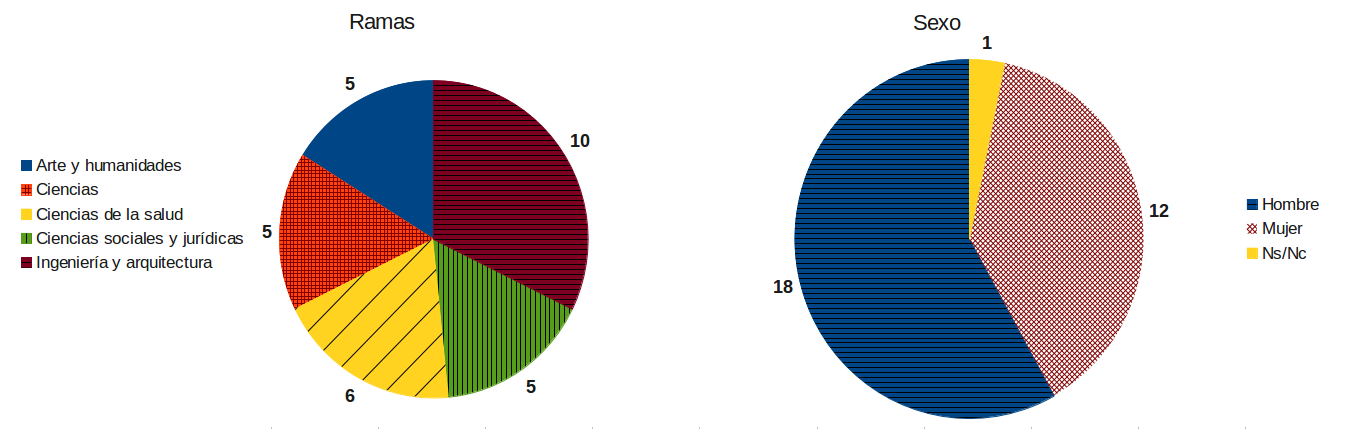
\includegraphics[scale=0.3]{JornadasPoblacion.png}
  \end{center}
  \caption{Distribución de los participantes por rama y sexo}
  \label{fig:cap:encuesta:ramaysexo}
\end{figure}


\begin{table}
  \begin{center}
  \begin{tabular}{| l | r | r | r | r |}
    \hline
    Rama \ Sexo & Hombre & Mujer & Ns/Nc & Total \\
    \hline
    \hline
    Arte y humanidades & 1 & 4 & 0 & 5  \\
    \hline
    Ciencias & 3 & 2 & 0 & 5  \\
    \hline
    Ciencias de la salud & 6 & 0 & 0 & 6  \\
    \hline
    Ciencias sociales y jurídicas & 2 & 2 & 1 & 5  \\
    \hline
    Ingeniería y arquitectura & 6 & 4 & 0 & 10 \\
    \hline
  \end{tabular}
\end{center}
\caption{Resumen de distribución de participantes por rama y sexo}
\label{tab:cap:encuesta:rama:sexo}
\end{table}

% LA PIE TIENE UN ESTILO DIFERENTE A LA DE POBLACIÓN DEL OTRO CUESTIONARIO (GDOC VS XLS). DEBERÍA UNIFICAR ...


\subsubsection{Evaluación del método DBA}

Para evaluar el método se preguntó a los docentes si consideraban el método DBA adecuado para obtener automáticamente indicadores de entornos de aprendizaje virtual. A esta pregunta fueron 26 de los 31 docentes encuestados (84\percentage) los que consideraron el método DBA adecuado (figura~\ref{fig:cap:encuesta:metodoDBA}).


\begin{figure}
  \begin{center}
    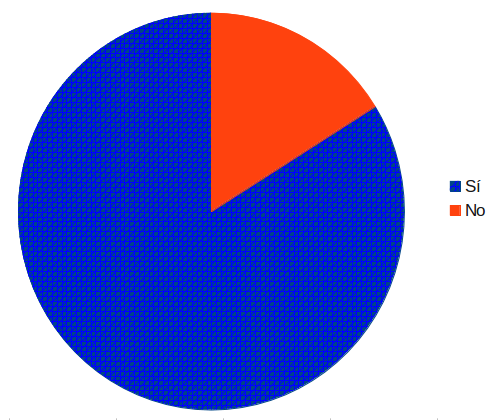
\includegraphics[scale=0.4]{EncuestaMetodoDBA.png}
  \end{center}
  \caption{Respuestas de los encuestados a la pregunta sobre el método DBA}
  \label{fig:cap:encuesta:metodoDBA}
\end{figure}

En general se puede decir que los docentes consideran el método como válido. Pero también es necesario determinar si existe relación entre la respuesta de cada docente y su rama. Para ello, se define como hipótesis nula que \emph{la consideración por parte de un docente de que el método DBA sea o no válido es independiente de la rama de dicho docente}. Para contrastar la hipótesis se utilizó el test de Fisher, no pudiéndose rechazar la hipótesis con un p-valor de 0,6142, muy superior al umbral de significación del 0,005.

Para afinar un poco más se decidió además agrupar los docentes según si pertenecen a las Ciencias natutales, Ciencias de la salud e Ingeniería (\emph{EHSE, Earth \& Health Sciences and Engineering}) o a Ciencias Sociales y Humanidades (\emph{SSH, Social Sciences and Humanities}). Para ello, se define como hipótesis nula que \emph{la consideración por parte de un docente de que el método DBA sea o no válido es independiente de si  dicho docente es de EHSE o de SSH}. Para contrastar la hipótesis se utilizó el test de Fisher, no pudiéndose rechazar la hipótesis con un p-valor de 0,2955, superior al umbral de significación del 0,005.

El resumen de las respuestas puede verse en la tabla~\ref{tab:cap:encuesta:metodoDBA:rama}.

\begin{table}
  \begin{center}
  \begin{tabular}{| l | l | r | r | r |}
    \hline
    & Rama & Sí & No & Total \\
    \hline
    \hline
    \multirow{2}{2.5cm}{SSH} & Arte y humanidades & 4 & 1 & 5  \\
    \cline{2-5}
    & Ciencias sociales y jurídicas & 3 & 2 & 5  \\
    \hline
    \multirow{3}{2.5cm}{EHSE} & Ciencias & 5 & 0 & 5  \\
    \cline{2-5}
    & Ciencias de la salud & 5 & 1 & 6  \\
    \cline{2-5}
    & Ingeniería y arquitectura & 9 & 1 & 10 \\
    \hline
  \end{tabular}
\end{center}
\caption{Consideración de idoneidad del método DBA por ramas}
\label{tab:cap:encuesta:metodoDBA:rama}
\end{table}

\paragraph{Características del método DBA}

Para continuar con la evaluación del método, se preguntó a los encuestados sobre su consideración acerca de en qué medida el método DBA satisface cada una de las características que se esperan del mismo. Estas características son \emph{objetividad}, \emph{adaptabilidad}, \emph{sistematicidad}, \emph{flexibilidad} y \emph{fiabilidad}. Para su evaluación se preguntó sobre ellos en una escala Likert de cinco puntos: totalmente de acuerdo, de acuerdo, ni de acuerdo ni en desacuerdo, en desacuerdo y totalmente en desacuerdo. 

En la tabla~\ref{tab:cap:encuesta:metodoDBA:caracteristicas} puede verse el porcentaje de votos que obtuvo cada uno de los puntos para cada característica. Las características de la \emph{adaptabilidad}, la \emph{sistematicidad} y la \emph{flexibilidad} son las más aceptadas para el método, ya que sumando los ''totalmente de acuerdo'' con los ''de acuerdo'' alcanzan más de la mitad de los votos, esto es, 61, 70 y 61\percentage{ }respectivamente. Mientras que sumando los ''en desacuerdo'' con los ''totalmente en desacuerdo'' tienen 16, 10 y 13\percentage{ }respectivamente. Por tanto, se podría decir que la mayoría de los docentes consideran que el método les proporciona estas características.

Para la \emph{objetividad} tenemos un 46\percentage{ }a favor (sumando los ''totalmente de acuerdo'' con los ''de acuerdo'') y un 22\percentage{ }en contra (sumando los ''en desacuerdo'' con los ''totalmente en desacuerdo''), mientras que para la \emph{fiabilidad} tenemos un 45\percentage{ }a favor y un 29\percentage{ }en contra, contando ambas características con un 26\percentage{ }de docentes que mantienen una opinión neutral, es decir, ni de acuerdo ni en desacuerdo. Por tanto, podemos decir que aunque con menor porcentaje de docentes a favor, tanto la \emph{objetividad} como la \emph{fiabilidad} son también aceptadas como características del método.

\begin{table}
  \begin{center}
  \begin{tabular}{| l | r | r | r | r | r |}
    \hline
    \multirow{3}{1.9cm}{Características} & \multirow{3}{1.9cm}{\centering Totalmente de acuerdo} & \multirow{3}{1.2cm}{\centering De acuerdo} & \multirow{3}{2.3cm}{\centering Ni de acuerdo ni en desacuerdo} & \multirow{3}{1.8cm}{\centering En desacuerdo} & \multirow{3}{1.9cm}{\centering Totalmente en desacuerdo} \\
    & & & & & \\
    & & & & & \\
    \hline
    \hline
    Objetividad & 23\percentage & 23\percentage & \textbf{32\percentage } & 19\percentage & 3\percentage \\
    \hline
    Adaptabilidad & 16\percentage & \textbf{45\percentage } & 23\percentage & 13\percentage & 3\percentage \\
    \hline
    Sistematicidad & \textbf{40\percentage } & 30\percentage & 20\percentage & 10\percentage & 0\percentage \\
    \hline
    Flexibilidad & 19\percentage & \textbf{42\percentage } & 26\percentage & 13\percentage & 0\percentage \\
    \hline
    Fiabilidad & 6\percentage & \textbf{39\percentage } & 26\percentage & 23\percentage & 6\percentage \\
    \hline
  \end{tabular}
\end{center}
\caption{Evaluación de las características del método DBA}
\label{tab:cap:encuesta:metodoDBA:caracteristicas}
\end{table}

\subsubsection{Evaluación del DSL}

Para evaluar el DSL se preguntó a los docentes si consideraban el lenguaje presentado útil para diseñar y contrastar estrategias de evaluación a partir de los registros de actividad de los entornos de aprendizaje virtual. A esta pregunta también fueron 26 de los 31 docentes encuestados (84\percentage) los que consideraron el lenguaje adecuado.

Por tanto se puede decir que los docentes consideran el método como válido. Pero también se quiso determinar si existía relación entre la respuesta de cada docente y su rama. Para ello, se define como hipótesis nula que \emph{la consideración por parte de un docente de que el lenguaje sea o no útil es independiente de la rama de dicho docente}. Para contrastar la hipótesis se utilizó el test de Fisher, no pudiéndose rechazar la hipótesis con un p-valor de 0,6142, muy superior al umbral de significación del 0,005.

Para afinar un poco más se decidió además agrupar los docentes según si pertenecen a las EHSE o a  las SSH. Para ello, se define como hipótesis nula que \emph{la consideración por parte de un docente de que el lenguaje sea o no válido es independiente de si  dicho docente es de EHSE o de SSH}. Para contrastar la hipótesis se utilizó el test de Fisher, no pudiéndose rechazar tampoco la hipótesis con un p-valor de 0,2955, superior al umbral de significación del 0,005.

El resumen de las respuestas puede verse en la tabla~\ref{tab:cap:encuesta:DSL:rama}.

\begin{table}
  \begin{center}
  \begin{tabular}{| l | l | r | r | r |}
    \hline
    & Rama & Sí & No & Total \\
    \hline
    \hline
    \multirow{2}{2.5cm}{SSH} & Arte y humanidades & 4 & 1 & 5  \\
    \cline{2-5}
    & Ciencias sociales y jurídicas & 3 & 2 & 5  \\
    \hline
    \multirow{3}{2.5cm}{EHSE} & Ciencias & 5 & 0 & 5  \\
    \cline{2-5}
    & Ciencias de la salud & 5 & 1 & 6  \\
    \cline{2-5}
    & Ingeniería y arquitectura & 9 & 1 & 10 \\
    \hline
  \end{tabular}
\end{center}
\caption{Consideración de idoneidad del DSL por ramas}
\label{tab:cap:encuesta:DSL:rama}
\end{table}

\paragraph{Características del DSL}

Para continuar con la evaluación del DSL, se preguntó a los encuestados sobre su consideración acerca de en qué medida el DSL satisface cada una de las características que se esperan del mismo. Estas características son \emph{facilidad de aprendizaje}, \emph{eficacia}, \emph{ahorra tiempo}, \emph{escalabilidad}, \emph{capacidad de reutilización} y \emph{fiabilidad}. Para su evaluación se preguntó sobre ellos en una escala Likert de cinco puntos: totalmente de acuerdo, de acuerdo, ni de acuerdo ni en desacuerdo, en desacuerdo y totalmente en desacuerdo. 

En la tabla~\ref{tab:cap:encuesta:DSL:caracteristicas} puede verse el porcentaje de votos que obtuvo cada uno de los puntos para cada característica. En primer lugar cabe destacar que el punto más votado en cuatro de las seis características fue el neutral, es decir, ni de acuerdo ni en desacuerdo. Estas cuatro características son la \emph{fiabilidad} con un 42\percentage, la \emph{facilidad de aprendizaje} con un 39\percentage, la \emph{escalabilidad} con un 35\percentage{ }y el \emph{ahorro de tiempo} con un 32\percentage{ }(en este último caso hay empate con el punto ''totalmente de acuerdo'').

A pesar de esta ''neutralidad'', también es importante resaltar que hay un bajo porcentaje de desacuerdos para las características, siendo todos los porcentajes inferiores al 20\percentage, excepto para la fiablidad que es un 23\percentage. Además, para todas las características son más los docentes que están de acuerdo que los que no, superando en cuatro de seis el 50\percentage{ }de votos a favor (\emph{facilidad de aprendizaje} con un 51\percentage, \emph{eficacia} con un 58\percentage, \emph{ahorro de tiempo} con un 55\percentage{ }y \emph{capacidad de reutilización} con un 58\percentage.

\begin{table}
  \begin{center}
  \begin{tabular}{| m{2.5cm} | r | r | r | r | r |}
    \hline
    \multirow{3}{2.5cm}{Características} & \multirow{3}{1.9cm}{\centering Totalmente de acuerdo} & \multirow{3}{1.2cm}{\centering De acuerdo} & \multirow{3}{2.3cm}{\centering Ni de acuerdo ni en desacuerdo} & \multirow{3}{1.8cm}{\centering En desacuerdo} & \multirow{3}{1.9cm}{\centering Totalmente en desacuerdo} \\
    & & & & & \\
    & & & & & \\
    \hline
    \hline
    Facilidad de aprendizaje & 19\percentage & 32\percentage & \textbf{39\percentage} & 7\percentage & 3\percentage \\
    \hline
    Eficacia & 13\percentage & \textbf{45\percentage} & 26\percentage & 16\percentage & 0\percentage \\
    \hline
    Ahorra tiempo & \textbf{32\percentage} & 23\percentage & \textbf{32\percentage} & 13\percentage & 0\percentage \\
    \hline
    Escalabilidad & 23\percentage & 23\percentage & \textbf{35\percentage} & 19\percentage & 0\percentage \\
    \hline
    Capacidad de reutilización & 26\percentage & \textbf{32\percentage} & 29\percentage & 6,5\percentage & 6,5\percentage \\
    \hline
    Fiabilidad & 6\percentage & 29\percentage & \textbf{42\percentage} & 23\percentage & 0\percentage \\
    \hline
  \end{tabular}
\end{center}
\caption{Evaluación de las características del DSL}
\label{tab:cap:encuesta:DSL:caracteristicas}
\end{table}

\subsubsection{Evaluación de la sintaxis del DSL (consulta tipo)}

Para evaluar la sintaxis del DSL se mostró una consulta de ejemplo y se preguntó a los docentes si consideraban la consulta entendible. A esta pregunta fueron 24 de los 31 docentes encuestados (77\percentage) los que consideraron entendible la consulta.

Por tanto se puede decir que los docentes consideran el método como válido. Pero también se quiso determinar si existía relación entre la respuesta de cada docente y su rama. Para ello, se define como hipótesis nula que \emph{la consideración por parte de un docente de que si la consulta es o no entendible es independiente de la rama de dicho docente}. Para contrastar la hipótesis se utilizó el test de Fisher, no pudiéndose rechazar la hipótesis con un p-valor de 0,121, superior al umbral de significación del 0,005.

Para afinar un poco más se decidió además agrupar los docentes según si pertenecen a las EHSE o a  las SSH. Para ello, se define como hipótesis nula que \emph{la consideración por parte de un docente de que la consulta es o no entendible es independiente de si  dicho docente es de EHSE o de SSH}. Para contrastar la hipótesis se utilizó el test de Fisher, no pudiéndose rechazar tampoco la hipótesis con un p-valor de 0,021, superior al umbral de significación del 0,005.

El resumen de las respuestas puede verse en la tabla~\ref{tab:cap:encuesta:consulta:rama}.

\begin{table}
  \begin{center}
  \begin{tabular}{| l | l | r | r | r |}
    \hline
    & Rama & Sí & No & Total \\
    \hline
    \hline
    \multirow{2}{2.5cm}{SSH} & Arte y humanidades & 2 & 3 & 5  \\
    \cline{2-5}
    & Ciencias sociales y jurídicas & 3 & 2 & 5  \\
    \hline
    \multirow{3}{2.5cm}{EHSE} & Ciencias & 5 & 0 & 5  \\
    \cline{2-5}
    & Ciencias de la salud & 5 & 1 & 6  \\
    \cline{2-5}
    & Ingeniería y arquitectura & 9 & 1 & 10 \\
    \hline
  \end{tabular}
\end{center}
\caption{Consideración de la consulta como entendible o no por ramas}
\label{tab:cap:encuesta:consulta:rama}
\end{table}

\subsubsection{Evaluación de los resultados}

Para evaluar los resultados devueltos por el DSL se mostró como ejemplo los resultados que devolvería la consulta de ejemplo y se preguntó a los docentes si consideraban dichos resultados entendibles. A esta pregunta fueron 20 de los 31 docentes encuestados (64\percentage) los que consideraron entendible la consulta.

Por tanto se puede decir que los docentes consideran el método como válido. Pero también se quiso determinar si existía relación entre la respuesta de cada docente y su rama. Para ello, se define como hipótesis nula que \emph{la consideración por parte de un docente de que si los resultados son o no entendibles es independiente de la rama de dicho docente}. Para contrastar la hipótesis se utilizó el test de Fisher, no pudiéndose rechazar la hipótesis con un p-valor de 0,010, superior al umbral de significación del 0,005.

Para afinar un poco más se decidió además agrupar los docentes según si pertenecen a las EHSE o a  las SSH. Para ello, se define como hipótesis nula que \emph{la consideración por parte de un docente de que los resultados son o no entendibles es independiente de si dicho docente es de EHSE o de SSH}. Para contrastar la hipótesis se utilizó el test de Fisher, no pudiéndose rechazar tampoco la hipótesis con un p-valor de 0,013, superior al umbral de significación del 0,005.

El resumen de las respuestas puede verse en la tabla~\ref{tab:cap:encuesta:resultados:rama}.

\begin{table}
  \begin{center}
  \begin{tabular}{| l | l | r | r | r |}
    \hline
    & Rama & Sí & No & Total \\
    \hline
    \hline
    \multirow{2}{2.5cm}{SSH} & Arte y humanidades & 3 & 2 & 5  \\
    \cline{2-5}
    & Ciencias sociales y jurídicas & 0 & 5 & 5  \\
    \hline
    \multirow{3}{2.5cm}{EHSE} & Ciencias & 5 & 0 & 5  \\
    \cline{2-5}
    & Ciencias de la salud & 5 & 1 & 6  \\
    \cline{2-5}
    & Ingeniería y arquitectura & 7 & 3 & 10 \\
    \hline
  \end{tabular}
\end{center}
\caption{Consideración de los resultados como entendibles o no por ramas}
\label{tab:cap:encuesta:resultados:rama}
\end{table}


\subsection{Resultados del cuestionario de indicadores}

El cuestionario (apéndice~\ref{Ap:cuestionario}) fue enviado en el mes de julio de 2015 a los diferentes colectivos. En este cuestionario se presentaba un estudio de caso de ejemplo en un wiki de Moodle, se mostraban dos consultas escritas en SASQL para la extracción de indicadores aplicables en la evaluación de competencias genéricas y se mostraban algunos de los indicadores y figuras obtenidas mediante la ejecución de dichas consultas en EvalCourse. 

En total se consiguieron 51 cuestionarios completados, cifra que consideramos adecuada a partir de la guía de Oates, que indica que 30 es el mínimo aceptado en una muestra adecuada para un primer proyecto de investigación. La distribución de los participantes con respecto a los grupos a los que pertenecen se muestra en la figura~\ref{fig:ResultadosParticipantes}.

\begin{figure}
  \begin{center}
    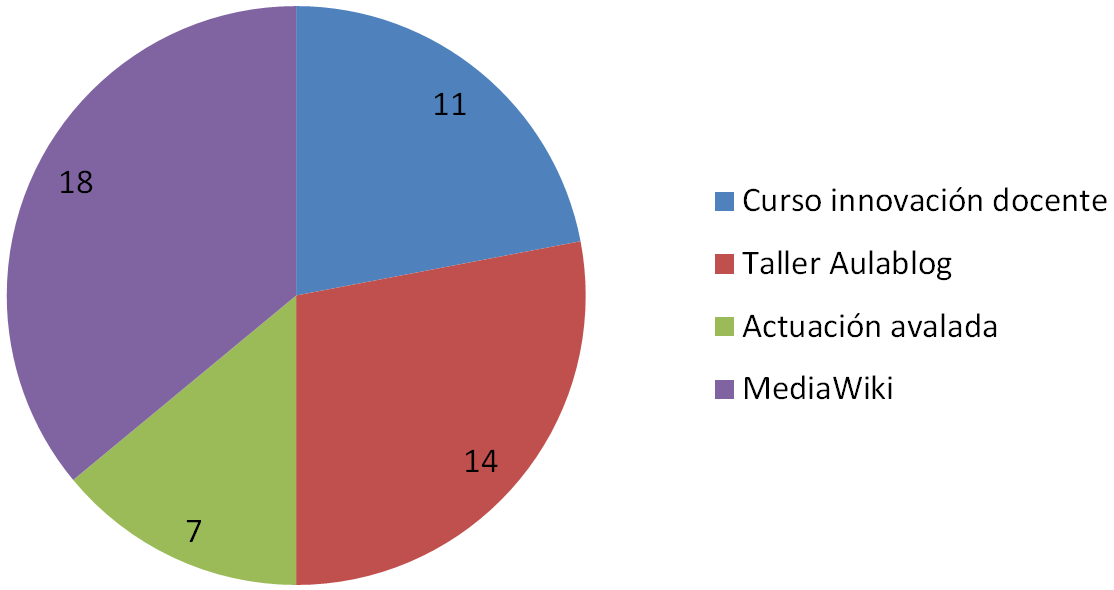
\includegraphics[scale=0.3]{ResultadosParticipantes.png}
  \end{center}
  \caption{Distribución de los participantes en el cuestionario}
  \label{fig:ResultadosParticipantes}
\end{figure}

\subsubsection{Perfil de los participantes}

El perfil de los participantes gira en torno a dos atributos. Estos atributos son los conocimientos de programación y la relación con la docencia. En la tabla~\ref{tab:eva:perfil} se muestra la distribución de los participantes en base a estos atributos.

\begin{table}
  \begin{center}
  \begin{tabular}{| c | m{3cm} | c | c | c | c | c |}
    \hline
     &  \multirow{3}{2cm}{\centering POBLACIÓN}  & \multirow{3}{1.7cm}{\centering Curso innovación docente}   & \multirow{3}{1.4cm}{\centering Taller Aulablog}  & \multirow{3}{1.55cm}{\centering  Actuación avalada} &  \multirow{3}{0.95cm}{\centering Media Wiki}  &  \multirow{3}{0.7cm}{\centering Total} \\
     &   &    &   &  &  &  \\
     &  &    &   &   &  &  \\
    \hline
    \hline
     \multirow{2}{2.5cm}{Conocimientos programación} & Nulos/básicos & 11 & 9 & 0 & 6 & 26 (51\percentage) \\
    \cline{2-7}
      & Medios/avanzados & 0 & 5 & 7 & 13 & 25 (49\percentage) \\
    \hline
	\hline
     & totales & 11 & 14 & 7 & 19 & 51 \\
	\hline
    \hline
     \multirow{3}{2.5cm}{Relación con la docencia} & Universitario & 11 & 2 & 7 & 1 & 21 (41\percentage) \\
    \cline{2-7}
      & No universitario & 0 & 12 & 0 & 0 & 12 (23\percentage)\\
    \cline{2-7}
     & No profesorado & 0 & 0 & 0 & 18 & 18 (35\percentage)\\
    \hline
  \end{tabular}
\end{center}
\caption{Perfil de los participantes que participaron en el cuestionario}
\label{tab:eva:perfil}
\end{table}

Con respecto a los conocimientos técnicos prácticamente hay un empate (26 con conocimientos nulos o básicos y 25 con conocimientos medios y avanzados). Hay que reseñar que fue necesario unir las respuestas de los participantes, ya que las poblaciones intermedias resultaron ser poco significativas y a la hora de aplicar estadísticos se requería un mínimo de población. Por eso los usuarios con conocimiento medio se unieron al grupo de los de conocimiento avanzado y los de conocimiento básico se unieron al grupo de los de conocimiento nulo.

Con respecto a la relación con la docencia vemos que también está repartido (25 docentes universitarios, 12 docentes no universitarios y 35 no docentes). En este caso ocurrió lo mismo. Los docentes no universitarios estaban repartidos entre docentes de infantil, primaria y secundaria. Estos grupos por separado resultaron ser muy poco significativos, por lo que se unieron también en un único grupo a fin de poder aplicar los estadísticos.

A partir de esta distribución de los usuarios se procede a evaluar la idoneidad del método y la herramienta para la evaluación de competencias genéricas en el siguiente apartado.

\subsubsection{Evaluación de competencias genéricas}

En el cuestionario se pregunta por, según el criterio del participante, la idoneidad de un conjunto de indicadores para evaluar las competencias genéricas del \emph{trabajo en equipo}, la \emph{planificación y gestión del tiempo} y el \emph{liderazgo}. El resumen de las respuestas dadas puede verse en la tabla~\ref{tab:eva::competencias}. 

\begin{table}
  \begin{center}
  \begin{tabular}{| c | c | c | c |}
    \hline
    RESPUESTA & Trabajo en equipo & Planificación y gestión del tiempo & Liderazgo \\
    \hline
    \hline
    Sí & 26 (51\percentage) & 40 (78,4\percentage) & 17 (33,3\percentage)  \\
    \hline
    No & 25 (49\percentage) & 11 (21,6\percentage) & 34 (66,7\percentage) \\
    \hline
  \end{tabular}
\end{center}
\caption{Resumen de la validez de cada indicador según los participantes en el cuestionario para evaluar cada competencia genérica}
\label{tab:eva::competencias}
\end{table}

Vemos que la tendencia de las respuestas de los participantes es diferente para cada competencia. Mientras que para evaluar el \emph{trabajo en equipo} podríamos decir que hay un empate entre el `sí` y el `no` (26 y 25 respectivamente), en la competencia de la \emph{planificación y gestión del tiempo} gana ampliamente el `sí` (40 a 11) y en la competencia del \emph{liderazgo} gana, aunque no tan ampliamente, el no (17 a 34). Como puede verse las cifras son diferentes para cada competencia, lo que viene a confirmar lo que se viene apostillando en esta tesis desde un principio. El indicador que es válido para un docente para evaluar competencias genéricas puede no serlo para otro. Para abordar ahora la independencia de las respuestas de los participantes en base a su perfil y sus conocimientos técnicos vamos a utilizar la prueba $\chi^2$ (\emph{chi cuadrado}) de Pearson. 

\paragraph{Independencia de las respuestas}

Para probar la independencia de las variables que intervienen en el cuestionario se utilizará la prueba $\chi^2$ de Pearson mediante la presentación de los datos en tablas de contingencia. Para cada competencia genérica se lanzaron dos hipótesis nulas. La primera con el objetivo de demostrar la independencia entre la respuesta de los participantes al uso o no de los indicadores y sus conocimientos de programación. La segunda para demostrar la independencia entre la respuesta y el perfil docente del participante. En total seis hipótesis nulas que fueron las siguientes:

\begin{enumerate}
\item Los \textbf{conocimientos de programación} son independientes de que el individuo considere que les son válidos los indicadores extraídos para medir la competencia de \textbf{trabajo en equipo}
\item Los \textbf{conocimientos de programación} son independientes de que el individuo considere que les son válidos los indicadores extraídos para medir la competencia de \textbf{planificación y gestión del tiempo}
\item Los \textbf{conocimientos de programación} son independientes de que el individuo considere que les son válidos los indicadores extraídos para medir la competencia de \textbf{liderazgo}
\item El \textbf{perfil en relación a la docencia} del individuo es independiente de que el individuo considere que les son válidos los indicadores extraídos para medir la competencia de \textbf{trabajo en equipo}
\item El \textbf{perfil en relación a la docencia} del individuo es independiente de que el individuo considere que les son válidos los indicadores extraídos para medir la competencia de \textbf{planificación y gestión del tiempo}
\item El \textbf{perfil en relación a la docencia} del individuo es independiente de que el individuo considere que les son válidos los indicadores extraídos para medir la competencia de \textbf{liderazgo}
\end{enumerate}

Se construyeron las tablas de contingencia, se calcularon las frecuencias esperadas y se obtuvieron los diferentes valores de $\chi^2$ para cada hipótesis. Una vez realizados los cálculos las hipótesis nulas 1, 2, 4, 5 y 6 no se rechazaron, concluyéndose que con una significación del 5\percentage{ }los datos son independientes. La hipótesis nula 3 sí quedaba rechazada con ese nivel de significación. Para no rechazarla el nivel de significación debía ser de un 0,1\percentage.

El estudio completo puede verse en la sección~\ref{apc:sec:resultados} del apéndice~\ref{Ap:cuestionario}.

\paragraph{Análisis de las justificaciones}

Los participantes en el cuestionario podían justificar con un comentario el porqué daban el `sí` o el `no` a la posibilidad de utilizar los indicadores a cada competencia. El listado de justificaciones completo puede verse en el apartado~\ref{ape:cuestionario:comentarios}. A continuación se resumen los justificaciones para cada competencia.

\paragraph*{Trabajo en equipo}

Los participantes que consideran que sí se puede evaluar el trabajo en equipo argumentan que los indicadores reflejan cómo se han coordinado los estudiantes, la periodicidad de sus contribuciones y sobre todo el volumen de lo aportado al trabajo.

Sin embargo, encontramos participantes que en estos indicadores sólo ven aportaciones individuales, y que demandan que para medir un trabajo en equipo necesitarían otro indicador que mida la interacción de los miembros, si ha habido un reparto de trabajo o si alguno está desempeñando algún rol.

\paragraph*{Planificación y gestión del tiempo}

En esta competencia el indicador que más defienden los participantes para evaluar el trabajo en equipo es la periodicidad de las contribuciones. De esta forman consideran que queda justificado si se ha distribuido el trabajo a lo largo del curso y por tanto se ha tenido una buena planificación.

En esta ocasión, los comentarios para no utilizar este indicador van en la línea de la falta de información previa. Es decir, para saber si se han planificado bien, tengo que saber de antemano en qué consistía el trabajo, cómo estaba organizado el curso, si pueden haber existido otros factores que hayan influido, etc. 

\paragraph*{Liderazgo}

Para justificar el liderazgo la mayoría de los participantes se basan en el nivel de participación, es decir, consideran que un estudiante ha ejercido un papel de liderazgo porque ha contribuido al wiki más que sus compañeros. Además, inciden en que el líder dedica al wiki más tiempo que sus compañeros, con contribuciones iniciales que animan a los demás, y con contribuciones finales, para corregir o supervisar el trabajo de estos.

Los participantes que abogan por el `no` se basan principalmente en que el nivel de participación no implica liderazgo, por lo que descartan totalmente el indicador proporcionado para medir el liderazgo. Se propone como alternativa opuesta que un indicador de liderazgo podría ser considerar precisamente qué usuario es el que menos trabaja, siendo necesario complementar este indicador con otro relativo a la comunicación entre los miembros del equipo.

\subsection{Resultados de la encuesta complementaria de indicadores}

Además del cuestionario principal, los docentes que participaron en los proyectos de actuación avalada recibieron un cuestionario en el que valoraban para qué competencias genéricas consideraban útiles los indicadores proporcionados por la herramienta EvalCourse (apéndice~\ref{Ap:cuestionarioAA}). Esta encuesta también tuvo lugar en julio de 2015, siendo 8 los docentes que participaron en la misma. La tabla~\ref{tab:indicador:competencia} muestra para cada competencia genérica (filas) cuántos docentes la consideraron evaluable a partir de alguno de los indicadores (columnas).

\begin{table}
	\centering
	\caption{Cuadro de indicadores considerados para cada competencia}
	\label{tab:indicador:competencia}
	\begin{tabular}{|m{3.8cm}|c|c|c|c|c|}
		\hline
		Competencia & Accesos & Foros & Actividades & Wiki & Talleres \\
		\hline
		\hline
		Trabajo en equipo & 1 & 2 & 2 & 4 & 0  \\
		\hline
		Planificación y gestión del tiempo & 5 & 2 & 6 & 5 & 0  \\
		\hline
		Razonamiento crítico y autocrítico & 0 & 4 & 2 & 1 & 0  \\
		\hline
		Capacidad para identificar, plantear y resolver problemas & 0 & 5 & 4 & 2 & 1 \\
		\hline
		Habilidades de interacción interpersonal & 2 & 6 & 0 & 3 & 1 \\
		\hline
		Trabajo autónomo & 6 & 3 & 5 & 7 & 1 \\
		\hline
	\end{tabular}
\end{table}

En este caso, los resultados vienen desglosados por cada actividad del campus virtual. Cabe destacar que la competencia genérica a la que más se pueden aplicar los indicadores de actividad del campus virtual para su evaluación según los docentes que participaron en la encuesta es el trabajo autónomo, seguida de la planificación y gestión del tiempo. En la sección~\ref{ape:AA:resultados} del apéndice~\ref{Ap:cuestionarioAA} pueden verse al completo las justificaciones de los docentes para considerar los registros de cada una de las actividades aquí indicadas como indicadores de competencias genéricas.

\subsection{Discusión y análisis}

Los resultados de los cuestionarios son muy satisfactorios. En primer lugar, se han evaluado el método DBA y el DSL que implementa el método, con el fin de medir la consecución de las hipótesis planteadas en esta tesis para medir la consecuión de los objetivos. En segundo lugar, se han evaluado los resultados obtenidos mediante el DSL, con el fin de valorar su aplicabilidad en la evaluación de diferentes competencias genéricas.

\paragraph*{Método DBA y DSL}
El 84\percentage{ }de los docentes encuestados consideran adecuado el método DBA para obtener indicadores de entornos de aprendizaje virtual y consideran el DSL útil para diseñar y contrastar estrategias de evaluación a partir de los registros de actividad de dichos entornos. 

A las encuestas se les pasó el test de Fisher para valorar si las respuestas de los docentes son independientes de la rama a la que pertenecen. No se pudo rechazar la hipótesis de independencia de las respuestas para ningún caso, quedando en ambos casos el estadístico muy por encima del valor umbral.

Para afinar aún más en el detalle, se volvió a realizar el test de Fisher tras agrupar a los docentes en dos grupos, según pertenezcan a las SSH (\emph{Social Science and Humanities}) o a las EHSE (\emph{Earth and Healt Science and Engineering}). En este caso, tampoco se pudo rechazar la hipótesis de independencia, quedando siempre el valor del estadístico por encima del valor umbral.

Además, el 77\percentage{ }considera entendible la sintaxis utilizada para definir las consultas en el DSL, mientras que el 64\% considera entendibles los resultados obtenidos a partir de la ejecución de dichas consultas.

También en estos casos se aplicó el test de Fisher para valorar la independencia de los resultados, primero con respecto a las ramas de los docentes y segundo con respecto al agrupamiento de dichas ramas según sean de SSH o de EHSE. En todos los casos, el estadístico quedó por encima del umbral, aunque no con una diferencia tan amplia como en los casos anteriores. Sobre todo es llamativo lo que ocurre con los resultados, donde todos los docentes del area de Ciencias Sociales marcaron como no entendibles los resultados que devolvía el DSL. A pesar de ello, se sigue sin poder rechazar la hipótesis de independencia.

Por tanto, a partir de los resultados obtenidos se acepta la consecución de las hipótesis planteadas en esta tesis:
\begin{itemize}
\item \emph{H1}: El método DBA permite obtener de manera automática indicadores de los entornos de aprendizaje virtual
\item \emph{H2}: El DSL permite a los docentes diseñar y contrastar estrategias de evaluación a partir de los registros de actividad de los entornos de aprendizaje virtual
\end{itemize}

Además, se ha preguntado a los encuestados tanto si el método DBA como el DSL han satisfecho las características que se les espera. 

Más de la mitad de los docentes (entre el 60 y el 70\percentage) considera que el método DBA satisface las características de la \emph{adaptabilidad}, \emph{sistematicidad} y la \emph{flexibilidad}. Las características de la \emph{objetividad} y la \emph{fiabilidad} también tienen un mayor porcentaje de votos a favor que en contra, aunque con menor porcentaje  (en torno al 45\percentage).

Con respecto a las características del DSL siguen siendo, para todas las características, más los docentes que están a favor que los que están en contra. Sin embargo, en torno un tercio de los encuestados para cada característica se situa en la posición neutra. Las características de la \emph{facilidad de aprendizaje}, la \emph{eficacia}, el \emph{ahorro de tiempo} y la \emph{capacidad de reutilización} tiene un porcentaje de docentes a favor de entre el 50 y el 58\percentage. La \emph{escalabilidad} cuenta con 46\percentage{ }a favor y la \emph{fiabilidad} con un 35\percentage. 

\paragraph*{Indicadores de competencias genéricas}
Aunque en esta tesis se propone un método y una herramienta para la evaluación de competencias genéricas, no es un objetivo de esta tesis establecer un indicador fehaciente para ninguna de ellas. Eso sería un objetivo más propio de investigación en ciencias sociales y de la educación. En los ejemplos mostrados se proponen ejemplos de indicadores, y según el criterio de cada participante en el cuestionario, unos son más válidos que otros. Para la competencia del \emph{trabajo en equipo} prácticamente hay un empate entre el `sí` (26) y el `no`(25). Mientras que en la \emph{planificación y gestión del tiempo} domina el `sí` (40 a 11), en la competencia del \emph{liderazgo} domina el `no` (17 a 34). Las justificaciones de los participantes en muchos casos para dar el `no` van en la línea de la necesidad de completar el indicador con información previa. Esto podría ser un ejercicio de redefinición de la hipótesis inicial o un rediseño de la evaluación.

%En segundo lugar, partiendo de los diferentes perfiles de los participantes en la encuesta se demuestra que sus respuestas son independientes tanto de su perfil docente como de su perfil más o menos técnico. De esta manera se descarta que las propuestas de diseño de evaluación de competencia genérica tengan una orientación demasiado técnica y que por tanto sean estos los únicos que acepten los diseños, o que esté más cercano a un docente de perfil universitario. El establecimiento de una serie de hipótesis nulas y la prueba $\chi^2$ de Pearson así lo han demostrado.

En segundo lugar, hay evidencias significativas a favor de que las respuestas de los participantes en la encuestas son independientes tanto del perfil docente como del perfil más o menos técnico de estos. A esta conclusión se llega después haber establecido una serie de hipótesis nulas y haber aplicado la prueba $\chi^2$ de Pearson. De esta manera se descarta que las propuestas de diseño de evaluación de competencia genérica tengan una orientación demasiado técnica y que por tanto sean los usuario con perfil técnico los únicos que acepten los diseños, o que esté más cercano a un docente de perfil universitario. 

Hay que comentar que el hecho de que la hipótesis nula número 3 fuese más difícil de demostrar tiene una explicación. La mayoría de los usuarios que dijo `sí` a la posibilidad de evaluar la competencia de liderazgo fueron los participantes en el curso de innovación y el taller de Aulablog. En dichas sesiones, con más interactividad que otras actuaciones, se mostraron ejemplos de cómo detectar a un usuario que ejercía una labor de liderazgo en un equipo de trabajo en wiki y esto pudo influir en el hecho de que a dichos participantes les costase menos interpretar en dichos indicadores la posibilidad de utilizarlos para realizar la evaluación que a otros. % innovación y el taller de Aulablog  (14 de los 17 síes).

El cuestionario complementario utilizado en la actuación avalada muestra que los docentes consideraron aplicar los indicadores obtenidos mediante EvalCourse en el campus virtual de Moodle a varias competencias genéricas. Las respuestas de los participantes difieren prácticamente para cada actividad y competencia genérica. Este hecho, al igual que la diferencia de criterio en las respuestas a `sí` y `no` a las competencias genéricas del cuestionario principal, respaldan aún más si cabe la propuesta de esta tesis doctoral, es decir, la necesidad de proponer este método a los docentes para que cada uno sea capaz de construir los indicadores que les sean válidos.

\section{Contribuciones} \label{eva:contribuciones}

	A continuación se indican las aportaciones principales que se han realizado durante la elaboración de este trabajo de investigación:



	\subsection*{Revistas}

	\begin{itemize}
	\item Artículo en la revista Computers in Human Behavior (2014), titulado ``Scalability of assessments of wiki-based learning experiences in higher education''~\cite{palomo2014scalability}.
	\end{itemize} 

\setlength{\fboxsep}{2pt}
\fcolorbox{grey}{grey}{\parbox{0.7\textwidth}{%
   \color{black}%
ISI JCR 2014: Q1, T1 (PSI, Multidisciplinary)
}}


	\begin{itemize}
	\item Artículo en la revista International Journal of Engineering Education (2015), titulado ``A Domain Specific Language for Online Learning Competence Assessments''~\cite{Balderas:2015}.

	%\item Artículo en la Revista Iberoamericana de Tecnologias del Aprendizaje (2015), titulado ``Learning Technologies and Semantic Integration of Learning Resources´´~\cite{dodero2015learning}.
	\end{itemize}

\fcolorbox{grey}{grey}{\parbox{0.7\textwidth}{%
   \color{black}%
ISI JCR 2014: Q3, T3 (Engineering, Multidisciplinary) \\
ISI JCR 2014: Q4, T3 (Education, Scientific Disciplines)
}}


	\subsection*{Congresos}

	\begin{itemize}
	\item Artículo presentado en el congreso IX Simposio Pluridisciplinar sobre Diseño, Evaluación y Descripción de Contenidos Educativos (SPDECE 2012), titulado ``Qualitative assessment of wiki-based learning processes''~\cite{Balderas:2012}.
	\item Artículo presentado en el I International Conference on Technological Ecosystem for Enhancing Multiculturality (TEEM 2013), titulado ``A generative computer language to customize online learning assessments''~\cite{balderas2013generative}.
	\item Artículo presentado en el International Symposium on Computers in Education (SIIE 2014), titulado ``Domain-driven competence assessment in virtual learning environments. Application to planning and time management skills''~\cite{balderas2014domain}.
	\item Artículo presentado en el III International Conference on Technological Ecosystem for Enhancing Multiculturality (TEEM 2015), titulado ``A Domain Specific Language to retrieve objective indicators for foreign language learning in virtual worlds''~\cite{balderas2015domain}.
	\item Artículo presentado en el  III Congreso Internacional Sobre Aprendizaje, Innovación y Competitividad (CINAIC 2015), titulado ``Evaluación del trabajo individual y grupal en un wiki''~\cite{reinoso2015evaluacion}.
	\end{itemize}


%\section{Conclusiones}
